\section{Evaluating the Adapted STEGO}\label{sec:proof-of-concept}
% experiments introduction
In a first step, the pre-trained models shipped with \gls{stego} were used to predict a selected data set (screws data set).
This could hint at a general transferability of models and was also used as base-line for comparisons with the second experiment, where \gls{stego} was trained on the screws data set with different cropping regimes.
Since \gls{stego}s loss function leverages the signal of similar and dissimilar features in images, and most scientific imaging experiments reproduce scans of the same object over and over again, trainings were done with different cropping regimes to artificially increase heterogeneity between slices.


\subsection{Methods}
In the following, an overview on the used methods is given.
The data set used for the experiments is introduced, and the experiments are explained.

\subsubsection{Data Set}
Both experiments were run on an in-house data set (screws data set), originally gathered to investigate how biodegradable bone implants (screws) are absorbed by the body after implantation~(\autoref{fig:screws-example}).
The aim of the segmentation was to differentiate between the labels \formatLabel{bone, degraded screw, screw} and \formatLabel{background} (also containing soft tissues).
A ground truth segmentation was available for all samples used.
The particular challenge of this data set was the label \formatLabel{degraded screw}, which was scarce in comparison to the other labels, so there was a pronounced imbalance between labels.
Additionally, pixels belonging to this label often had very similar pixel values and also textures as the \formatLabel{screw} label.
So overall, it was mostly distinguished through its borders, and did not consist of homogenous pixels.
This data set has been used before with a supervised learning approach~\autocite{Baltruschat2021}, so a direct comparison of the model performance can be made.

The data set consisted of 17 3D high resolution \gls{srmct} scans of magnesium alloy screws in bone, that were either made at the P05 imaging beamline at \gls{desy} or at the Diamond Manchester Imaging Branchline I13-2.
Afterwards, volumes were resampled with bi-linear interpolation to a fixed voxel-size of 5~µm, clipped to a dynamic range of 0.5 and 99.9~\% and normalised, so grey-values are in the range [0,1].
Each volume was cropped to a size of $1200 \times 1200 \times 1000$~px.
The ground truth of the samples was obtained via a time-consuming semi-automatic workflow, based on watershed segmentation.
14 of the semi-automatically segmented samples were used as train set (of which three were used for validation in each fold during five-fold cross-validation).
The remaining three samples were used for predictions only\footnote{Predicted volumes were: 113734HQMg5, syn009HQ, and 113729HQMg5.}.
For these three volumes, high quality segmentations were available done by an expert, who manually corrected the semi-automatic segmentation.
For more details on beam intensity, image reconstruction, and ground truth workflow see~\autocite{Baltruschat2021}.

\begin{figure}[!htb]
    \centering
    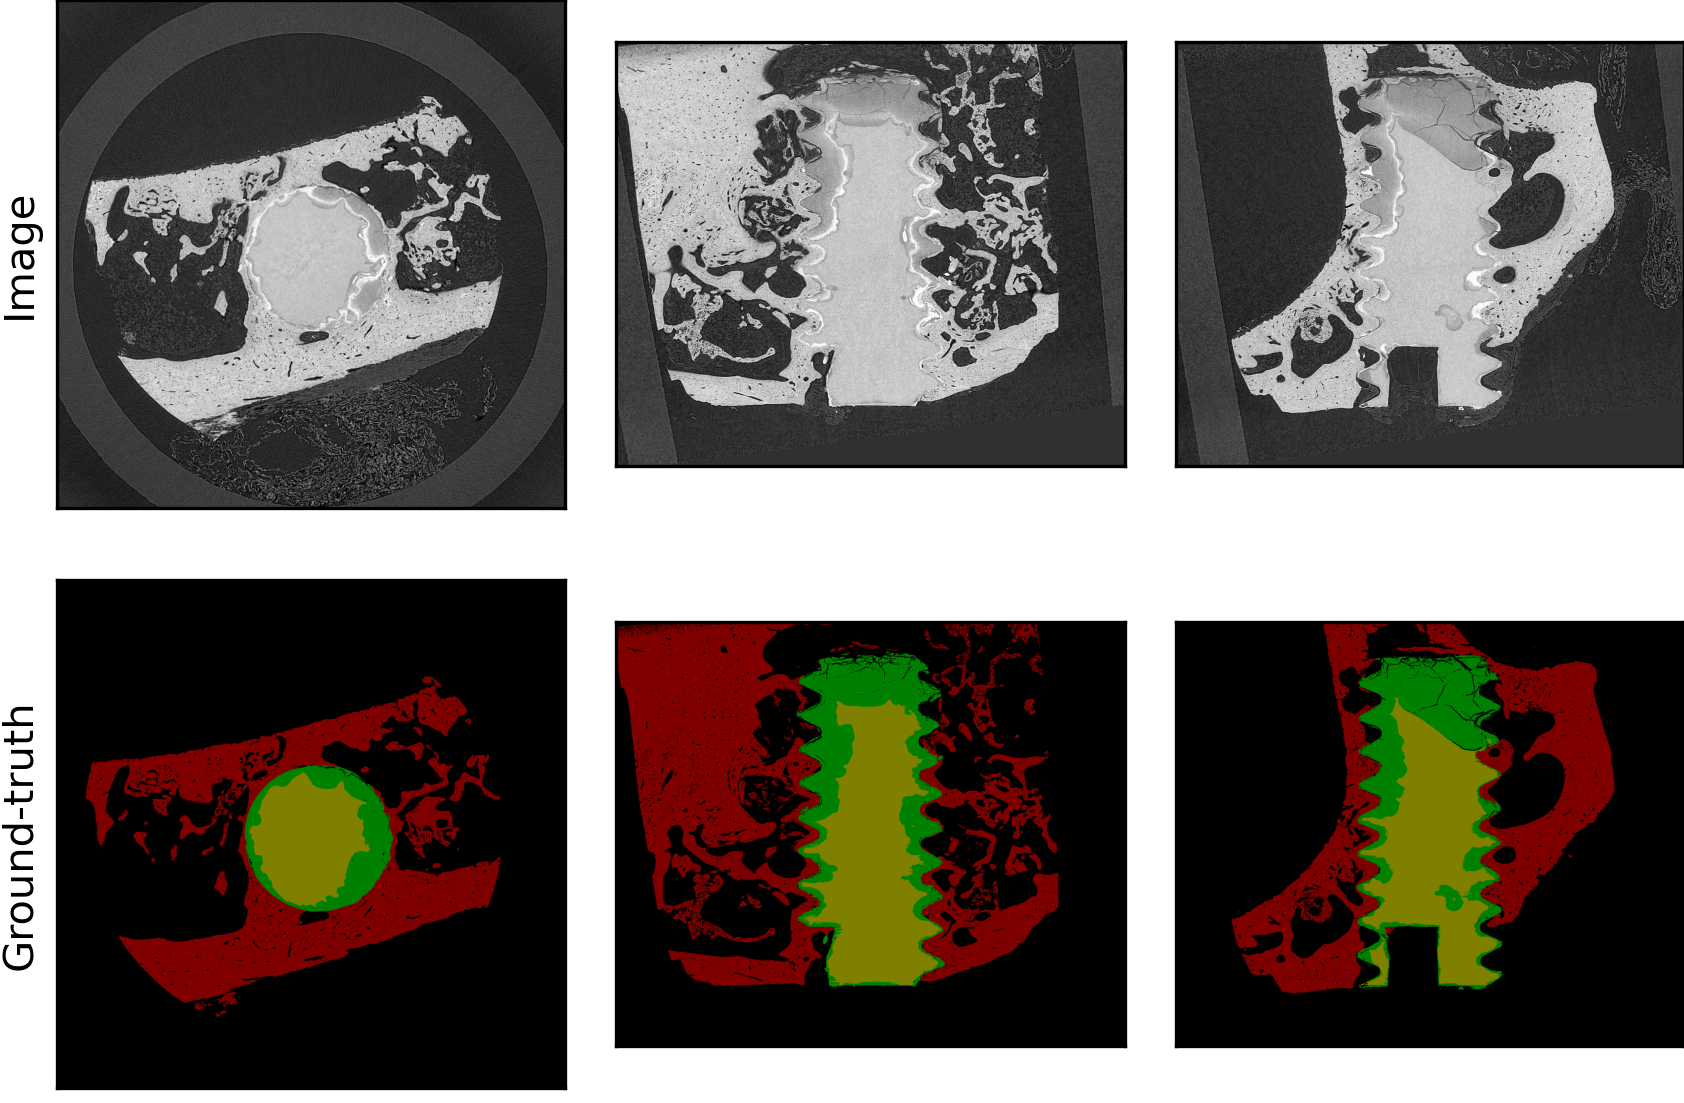
\includegraphics[width=\textwidth]{pictures/ExampleImageGroundtruth_syn009_slice500_allDirections}\\
    \caption[Example Images of Screws Data Set]{Example of images and ground truth segmentation of the screw data set. Slice 500 in every direction of volume syn009HQ is shown. The label color map is as follows: \formatLabel{background}: black, \formatLabel{bone}: red, \formatLabel{degraded screw}: green, \formatLabel{screw}: yellow.}
    \label{fig:screws-example}
\end{figure}

%\paragraph{Amber}
%The second data set used in the experiments consists of 19 \gls{srmct} image volumes of amber with arachnid inclusions.
% http://www.panarthropoda.de/sub/allgemeines/pseudoskorpioneen.php
%This data set was originally assembled to visualize the enclosed pseudoscorpions\footnote{Pseudoscorpions are a very old group of arachnids, resembling scorpions and reach sizes between 2 to 10~mm~\autocite{Harvey2002}.}
%Voxel-size was 2.4~µm, but image volumes vary in size, depending on size of the inclusion.
%The biggest volume is $1469 \times 1239 \times 1443~px$, the smallest $626 \times  348 \times  458~px$.
%By varying the slicing direction, the image slices could be brought to a minimal size of $626 \times 458~px$ and maximal size of $1239 \times 1443 px$.

% describe were images come from
%SRµCT images were obtained at \gls{desy}, at the storage ring PETRA III, Beamline P05.
%The attenuation contrast was conducted with an energy of 25~keV, the number of projections was 1200, and voxel size 2.4~µm.
%Scan time was about 2 hours for each scan.
%Projections were reconstructed to 32-bit floating point image stacks with the tomographic reconstruction algorithm ‘gridrec’.
%Ground truth segmentation of the scans was done manually for 12 of the 19 volumes in Amira (Thermo Scientific, 2016). % and took about 15 hours for each scan.
%First rough segmentation of the specimens was done via threshold selection, but completion had to be done manually.
%Especially bubbles and other impurities often had to be separated from the specimen manually slice by slice.

%\begin{figure}[!htb]
%    \centering
%    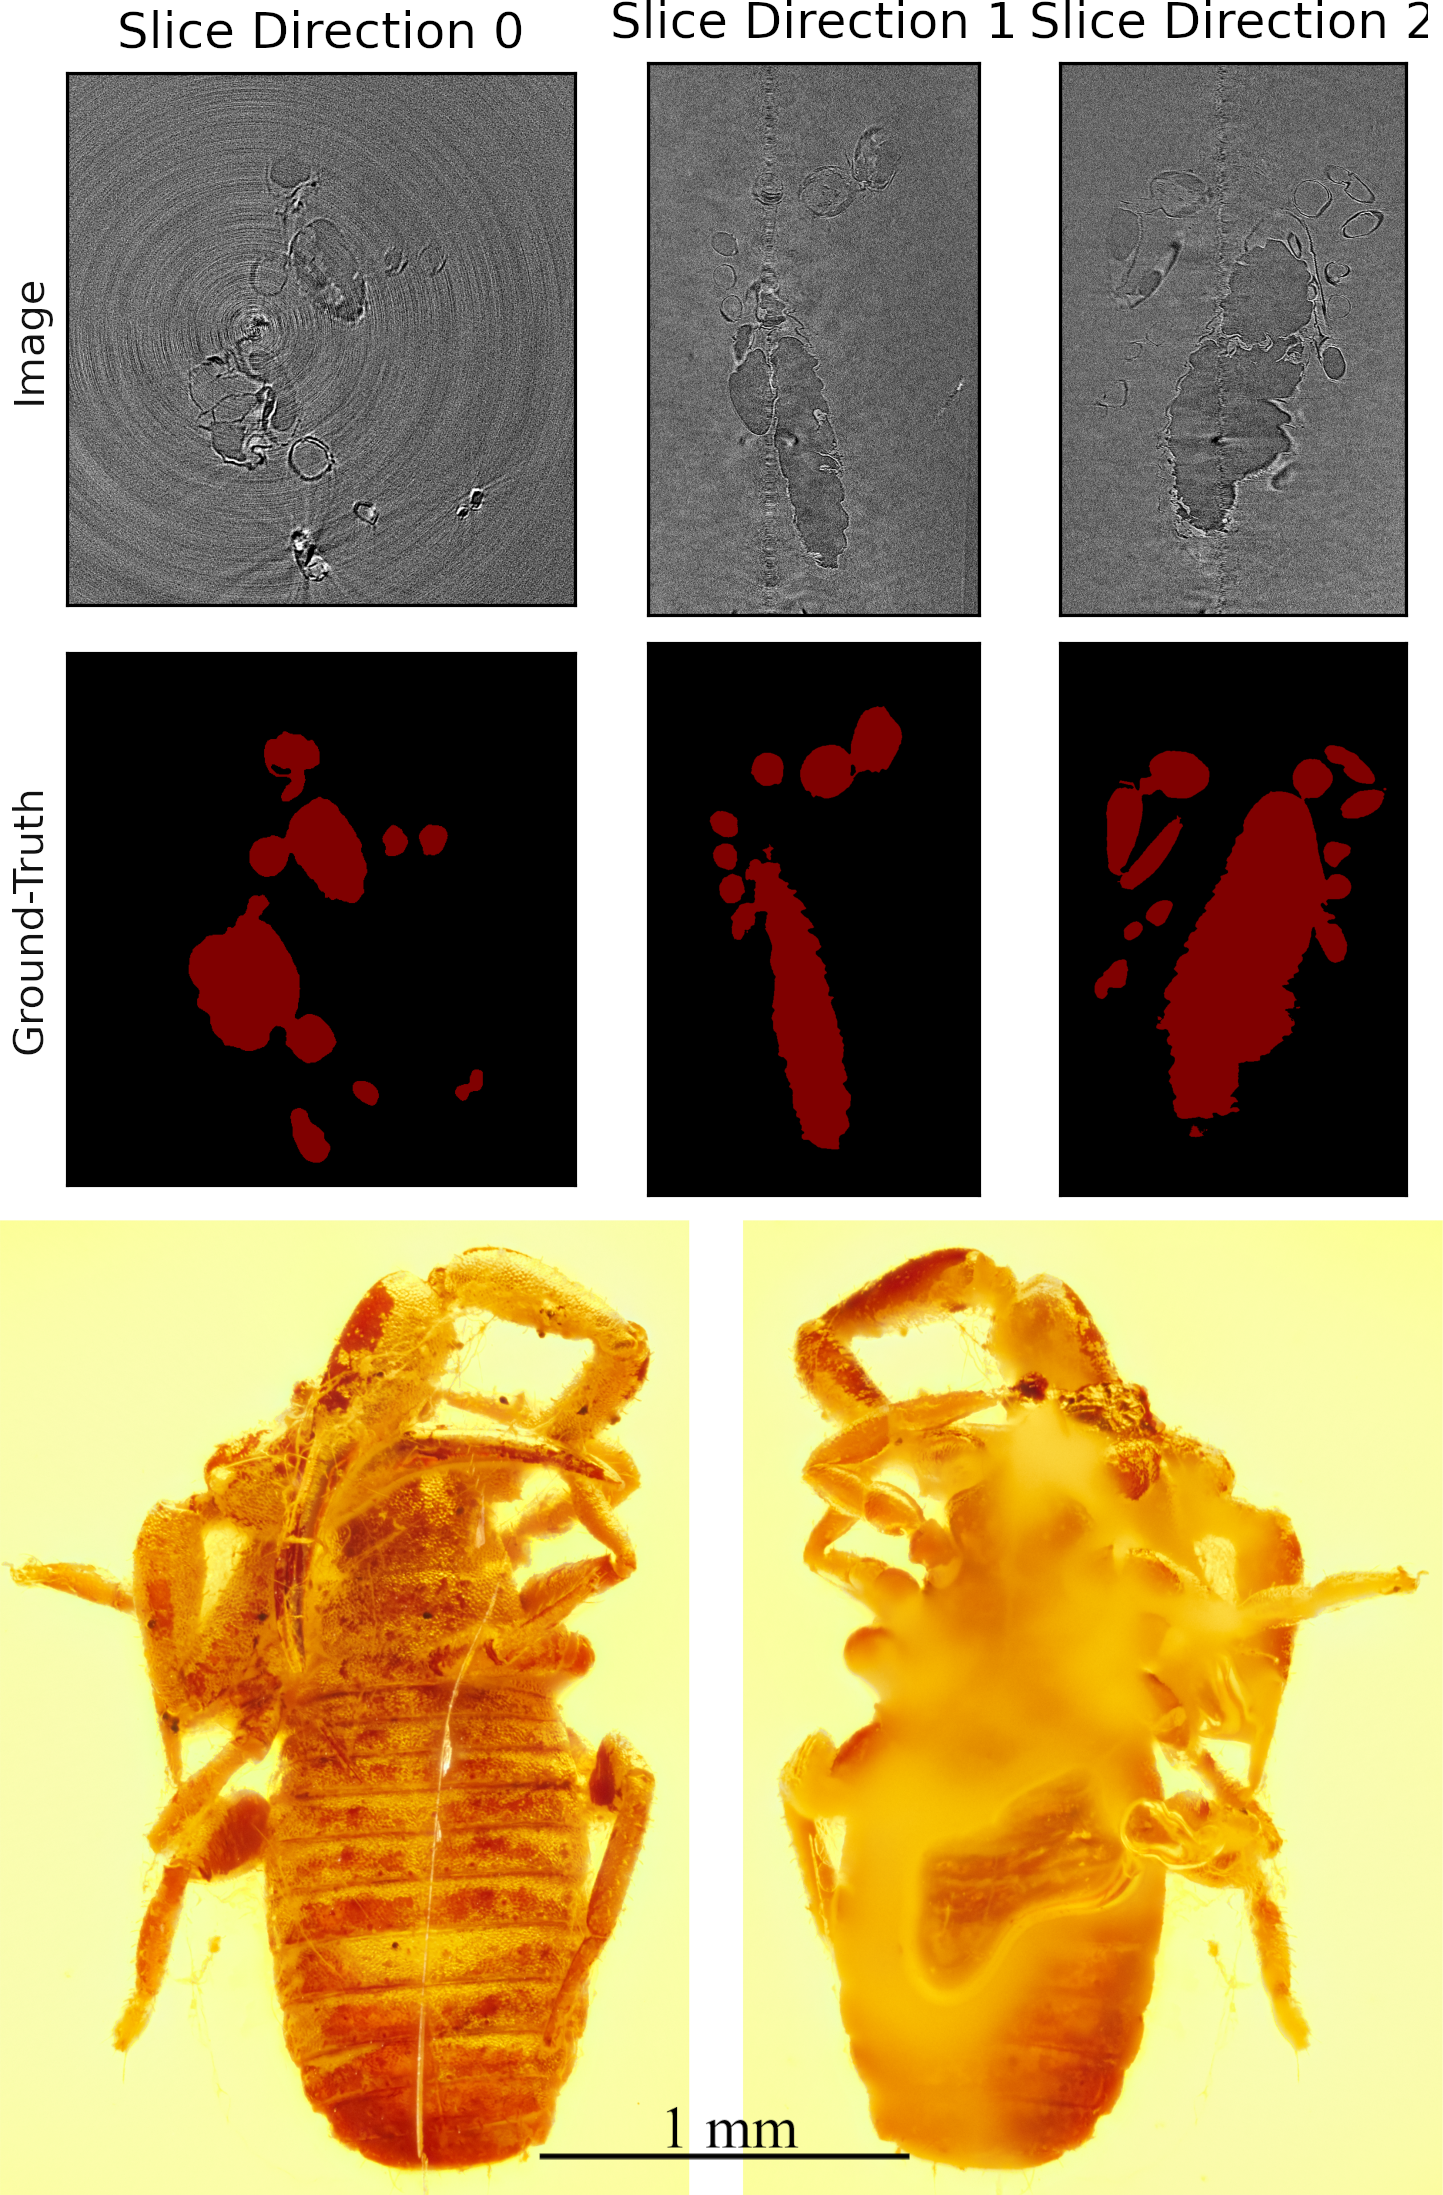
\includegraphics[width=0.95\textwidth]{pictures/Segmentation_Photo_PS-4}\\
%    \caption[Example Images and photograph of Amber Specimen]{Example of an amber specimen with image, ground truth and dorsal and ventral high resolution photograph. As seen part of the ventral side is hidden from visual inspection due to white emulsion leaked from the specimen and bubbles in the amber piece.}
%    \label{fig:amber-example}
%\end{figure}

%\paragraph{Mixed Data set}
%Both mentioned data sets (screws and amber) were combined into a mixed data set, with roughly the same number of images from amber and screws set.
%From the screw data set, which is much bigger than the amber set, 23.491~images were randomly selected from the five-cropped set (where image size nearly matches image size of the smallest amber slices), so the resulting mixed data set contained the same amount of images from the amber and screws set.
%Since the amber images were of variable sizes, the mixed data set should only be used center cropped to the smallest resolution ($458 \times 458~px$).
%This means loosing some information of lager amber images, and loosing some border pixels of the five-cropped screws images.
%However, since the amber data is just used to increase heterogeneity of the screws data set, and the aim of the data set is to enhance the screws predictions, not amber predictions, this should not be a problem.\footnote{Another option would have been to divide the bigger amber images in smaller slices to retain more of the amber information and adjust the number of screws images selected accordingly, but for simplicity this is not done here. Nevertheless, in future work, this should be investigated.}
%Because ground truth labels were not available for all amber volumes and the experiments designed for this data set aim at improving predictions of the screws, the train-validate-test-split of the mixed data set was done in a way that the validation and test sets match the screws data set. 
%Amber images were only added to the training set.
%To account for the five-fold cross validation, the amber images thus were partitioned into folds separately from the screws images and added to the training folds of the screws images.
%Slices belonging to the same volume were always kept in the same fold.
%Volumes were distributed between folds, so that every fold contains nearly the same number of slices.
%For the amber folds this means a slight variety of number of slices per fold: 4405, 4406, 4407, 4423, and 4381.
% 1. select x random images form five-fold screws trainset (all folds), to match number of amber pictures
% 2. make a five-fold cross validation of the selected screws images
% 3. partition amber into 5 folds of same size (keep volumes together) and add them to the screws train folds
% 4. copy test set of screws data set (since no changes here)

%\subsubsection{Experiments}
%To asses the capacity of the original \gls{stego}, and also to get a first feel for the potential of \gls{stego} for scientific data, in the first experiment the screws test data set was predicted with the pre-trained models \gls{stego} provides.
%Experiment two was designed to determine if and how training \gls{stego} on very homogenous data sets is yielding satisfactory results.
%This is done by using different cropping regimes, and hyper parameter combinations.

\subsubsection{Experiment 1: Predict with Provided Models}
To get a first feel for the capacity of \gls{stego}, the three volumes selected for predictions of the screws data set were predicted with the provided pre-trained models.
If the pre-trained models were found to predict the test data set quite well, this would hint at extraordinary transferability and generalisation capacity of \gls{stego}.


%used models
Three pre-trained models were provided by the authors of \gls{stego}.
A model trained on aerial photographs of Potsdam\footnote{\url{https://www.isprs.org/education/benchmarks/UrbanSemLab/2d-sem-label-Potsdam.aspx} (visited 15/02/2023)} resolving three (of the six original) classes, the COCO-Stuff\footnote{\url{https://github.com/nightrome/Cocostuff} (visited 15/02/2023)} model, which was trained on the COCO-Stuff data set and resolves 27 classes, and a model trained on the Cityscapes data set\footnote{\url{https://www.Cityscapes-dataset.com} (visited 15/02/2023)}, also resolving 27 classes.~\autocite{Hamilton2022}

%data sets of models
The Potsdam data set was released by ISPRS Commission WG II/4.
It consists of 38 aerial photographs of the city op Potsdam, with six categories to be differentiated (\formatLabel{impervious surface, building, low vegetation, tree, car, clutter}).
In the pre-trained \gls{stego} model, only the categories \formatLabel{roads and cars}, \formatLabel{buildings and clutter}, and \formatLabel{vegetation and trees} were used.
The COCO-Stuff data set augments the large-scale COCO (Common Objects in Context) data set with pixel-level stuff annotations.
Thus, semantic classes can be objects with well-defined shapes as in COCO (e.g.~\formatLabel{car, person}) or stuff (amorphous background regions, e.g.~\formatLabel{grass, sky}).
Cityscapes is a large-scale data set, that contains a diverse set of images of urban street scenes from 50 different cities.
Categories in the data set include: \formatLabel{person, bus, building, sidewalk, vegetation, tunnel} etc.
This means, there is some overlap in the categories between COCO-Stuff and Cityscapes.~\autocite{Hamilton2022}

% execution of experiment
%cropping vs scaling
Since the selected test data had a very high resolution, the images could not be loaded in full resolution.
Even with a batch size of one, computing nodes quickly run out of memory.
Therefore, images needed to be reduced, either scaled or center-cropped.
Since in \gls{srmct} minor details matter, images were cropped.
% experimenal set-up
So, the predictions were made on the center-cropped images (to $800 \times 800~px$) with each given model.
This means, a 200~pixels wide stripe was missing on each side of the original slide ($1200 \times 1200~px$ resolution).
Since the region of interest was centred in the images and this outer border mostly contained background (and some bone pixels), loosing the outer border was tolerable for this data set.
% evaluation of predictions
Predictions were evaluated using the Hungarian matching algorithm on the found clusters and ground truth labels, as proposed by \gls{stego}s authors.
By utilising the correlation values of the predicted clusters and ground truth labels, it could be determined to which ground truth label a cluster most likely belonged.
For the COCO-Stuff predictions, a manual assignment was additionally done, as explained later.
After combining clusters according to the most likely ground truth label, evaluation was run again to calculate~\gls{iou} between combined clusters and ground truth labels.

%expectations for experiment
When predicting with the pre-trained models, it was not expected that a perfect match is achieved.
For example, the Potsdam model only contains three classes, thus at least one class can not be resolved for the test cases evaluated here, since they contain four different labels.
The label not resolved will probably be the \formatLabel{degraded screw} label, since it is very similar to \formatLabel{screw} and will likely cluster with it at such broad categorisations.
However, it is still expected that the Potsdam model might perform relatively well, since the aerial images used for training are more similar to the test data than the training data of the other two models.
Still, the comparison of the models both resolving 27 classes will give valuable insights on the clustering capacities of \gls{stego}.


\subsubsection{Experiment 2: Train on a Scientific Data Set}
Since \gls{stego} utilises differences and similarities within the train set, the question arises, if (and how) it can be used on very homogenous data, as often found in scientific imaging.
To investigate this, image size and section was changed between trainings, since selecting different parts of images (e.g.~through random cropping) might lead to slightly more heterogeneity between training images.
To compare changes, a base model was trained on the five-cropped data set as recommended by \gls{stego}s authors.

% experimental set up: base-case
Training of the base case was done on the five-cropped screws data set.
Image size after cropping was $496 \times 496~px$, so most parts of the images were used (except for some pixels at the edges\footnote{Since the region of interest is centered in the images, this is tolerable.}).
Cropped images were loaded at full resolution for training and training was run for at least 20 epochs with a five-fold cross-validation.
The split of the data set into the five folds can be found in~\autoref{subsec:cross-validation-screws}.

%experimental set up: random cropping
Training on the random cropped data set was done the same way, but with different image sizes: medium size ($200 \times 200~px$)\footnote{Using the same size as with five-cropping would not change the data set significantly, so it was decided to train with less than half the image size.} and smaller crops ($96 \times 96~px$), since it was suspected that smaller crops might benefit the data set heterogeneity, as not all labels are included in every image.

% LOO + extra clusters
Two additional configurations were run:
To investigate the divergence of folds, a leave-one-out cross-validation was run on the base case, and different overclustering schemes were run (again on the base case) to better resolve the \formatLabel{degraded screw} label, which was found to perform poorly.
The assignment of volumes to the leave-one-out train and test set can be found in~\autoref{subsec:cross-validation-screws}.


% parameters used
The hyperparameters for the loss function, controlling the weights and shifts of the positive and negative signals, were tuned according to the recommendations by \gls{stego}s authors.
However, it was found that for the chosen data set a different weight ratio than recommended performed best.\footnote{The weight ratio recommended by the authors was $\neginter \sim \posintra \sim 2~\posinter$, but they differed from this ratio in their experiments, too~\autocite{Hamilton2022}.}
The weight ratio was set to $\neginter \sim \posintra \sim~0.5~\posinter$, a full list on parameters used can be found in~\autoref{tab:training-parameters}.
%It was also determined in preliminary experiments, that adjusting the learning rate, or changing the number of nearest neighbours to chose from for the positive signal did not improve performance, so \gls{stego} was used as-is, with the sole exception that number of steps was increased.
All trainings were done for 20 epochs using the \gls{desy} high-performance computing cluster Maxwell on computing nodes with four NVIDIA V100 GPUs.
Validation was run every 250 steps.

\subsection{Results}
Results are reported separately for experiment 1 (predictions of scientific images with the pre-trained models), and experiment 2 (training done on a scientific data set).

\subsubsection{Experiment 1: Predict with Provided Models}
In the following, models will be identified by the data set they were trained on.
Examples of original cluster predictions and predictions with clusters mapped to their most likely ground truth label can be found in~\autoref{fig:pretrained-predictions}.

\begin{figure}[p]
    \centering
    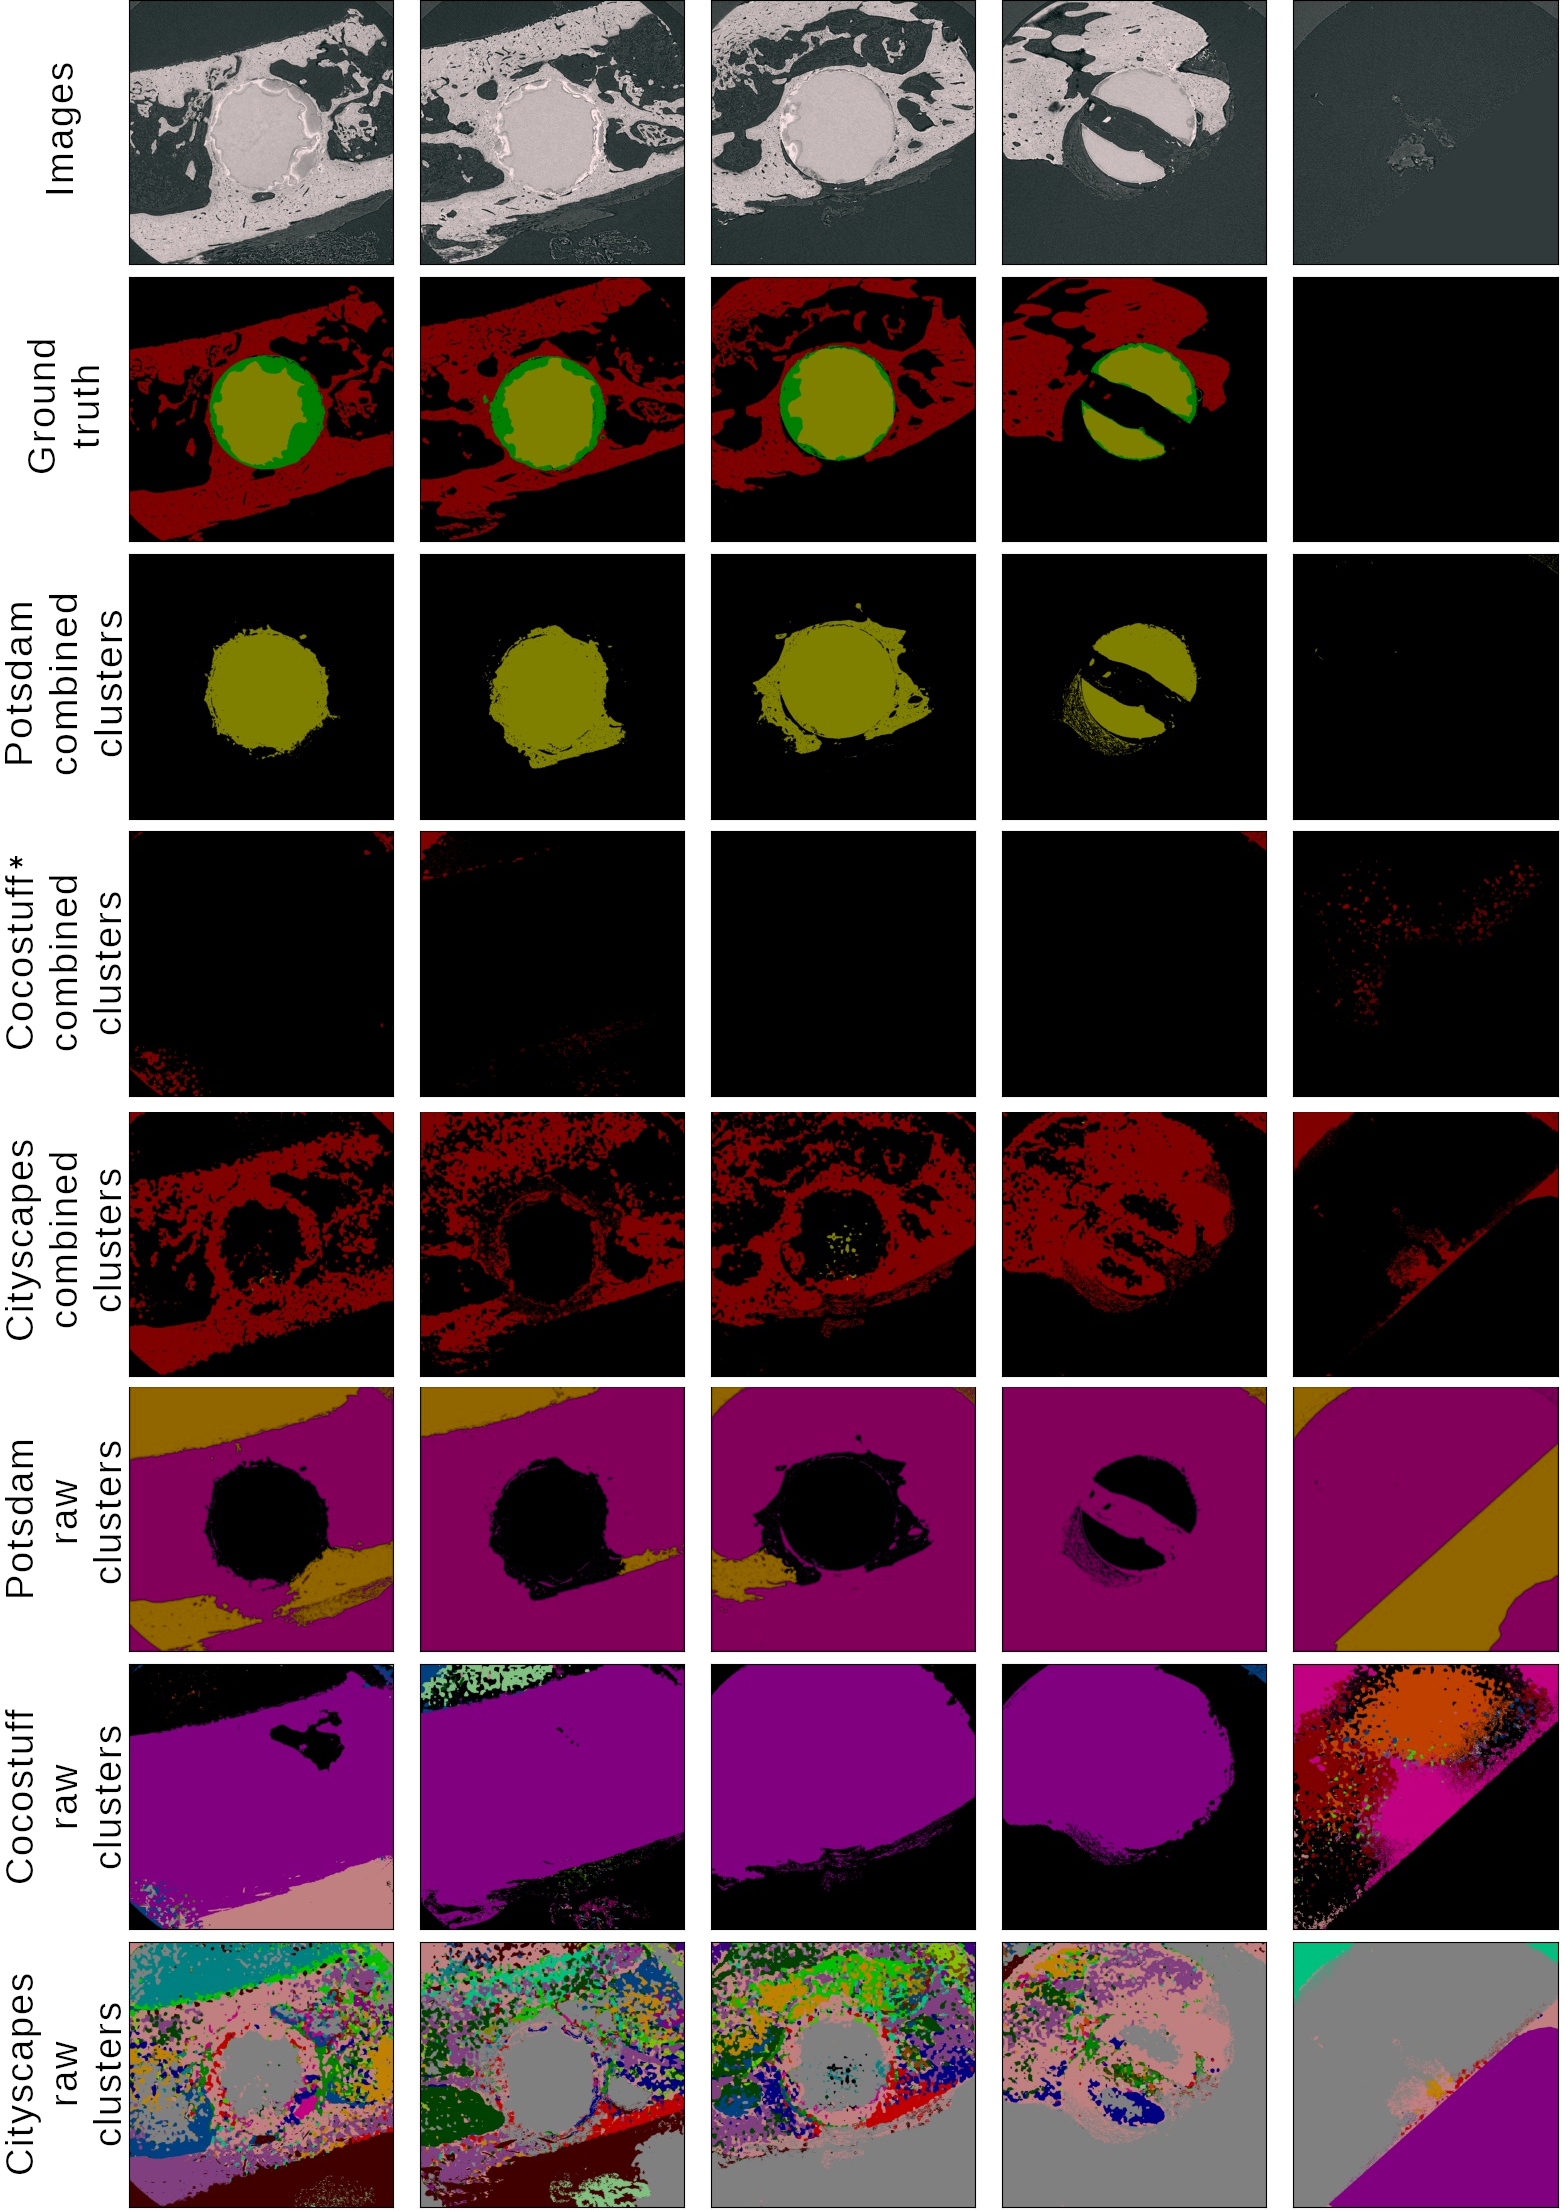
\includegraphics[width=\textwidth]{pictures/experiment_1/pretrained-models_cluster-predictions_example_predictions_2_small}\\
    \caption[Example Predictions from Provided Models]{Visualisation of image, ground truth, raw cluster predictions and clusters combined by their most likely match to ground truth label. Raw cluster colors correspond to cluster names in~\autoref{fig:correlation-matrix-pretrained}. Combined cluster assignment to ground truth labels is indicated by color. All shown slices belong to the second half of volume syn009HQ and are ordered according to spatial location in the volume. Every 100th slice is shown.
    \\ \textsuperscript{*}For more representative slices of combined clusters for COCO-Stuff see~\autoref{fig:more-cocostuff-predictions}.}
    \label{fig:pretrained-predictions}
\end{figure}

\begin{table}[!htb]
    \caption[IoU for Predictons with Pre-trained Models]{IoU of predicts done with pre-trained models. Predictions were made with different models, as identified by train data set (rows) for the same test set of the screws model. For each model, IoU of the ground truth label to the combination of clusters matching best according to correlation value is given (with manual corrections for COCO-Stuff), as well as the mean over all labels. A dash indicates that the label was not predicted. All values are rounded to the second decimal.}
    \label{tab:miou-pretrained-models}
    \makegapedcells      % in makecell
    \begin{tabular}{|>{\bfseries}l|c|c|c|c||c|}
        \hline
        Model & \textbf{\formatLabel{background}} & \textbf{\formatLabel{bone~~~}} & \makecell{\textbf{\formatLabel{degraded}}\\ \textbf{\formatLabel{screw}}} & \textbf{\formatLabel{screw}} & \textbf{mean} \\ \hline
        Potsdam & 0.71 & - & - & 0.36 & 0.27 \\ \hline
        Cocostuff & \makecell{0.69 \\(0.63)} & \makecell{0.35 \\(0.44)} & \makecell{0.00 \\(0.00)} & - & \makecell{0.26 \\(0.27)}\\ \hline
        Cityscapes & 0.65 & 0.37 &  - & 0.00 & 0.26\\ \hline
    \end{tabular}
\end{table}

%Potsdam
% model cluster to label assignment
% 0: buildings and clutter         -> screw
% 1: trees and vegetation          -> background
% 2: roads and cars                -> background
% cluster to label mapping
With the Potsdam model, the highest correlation was found between the Potsdam label \formatLabel{trees and vegetation} and \formatLabel{background} of the screws data set, though some \formatLabel{bone} pixels are also included (see~\autoref{fig:correlation-matrix-pretrained}).
Similarly, \formatLabel{roads and cars} correlated highly with \formatLabel{background} and to some degree also with \formatLabel{bone}.
The \formatLabel{buildings and clutter} cluster correlated to \formatLabel{screw} and and nearly to the same degree to \formatLabel{degraded screw} (in fact, all \formatLabel{screw} and \formatLabel{degraded screw} pixels were found in this cluster) and \formatLabel{bone}.
Additionally, \formatLabel{buildings and clutter} also contained \formatLabel{bone} and a few \formatLabel{background} pixels.
The other ground truth labels do not match as clearly, as seen in~\autoref{fig:correlation-matrix-pretrained}.

% combined clusters
When clusters were combined according to their most likely ground truth match (as seen in~\autoref{fig:correlation-matrix-pretrained}), Potsdam reached a slightly better overall \gls{miou} on the combined clusters and also the best \gls{iou} for a single label (\formatLabel{background} reached a \gls{miou} of 0.71), see ~\autoref{tab:miou-pretrained-models}.
% mIoU
\formatLabel{Bone} and \formatLabel{degraded screw} were not detected since no cluster correlated to them as clearly, and \formatLabel{screw} reached a \gls{iou} of 0.36.
When considering the predictions ~(\autoref{fig:pretrained-predictions}), the model mostly distinguishes two classes, one including \formatLabel{background} and \formatLabel{bone}, and one containing \formatLabel{screw} and \formatLabel{degraded screw}.
The differentiation between \formatLabel{screw/degraded screw} and \formatLabel{background/bone} was even visible in the fine cracks of the screw, as seen in~\autoref{fig:pretrained-predictions_syn009}.

\begin{figure}[!htb]
    \centering
    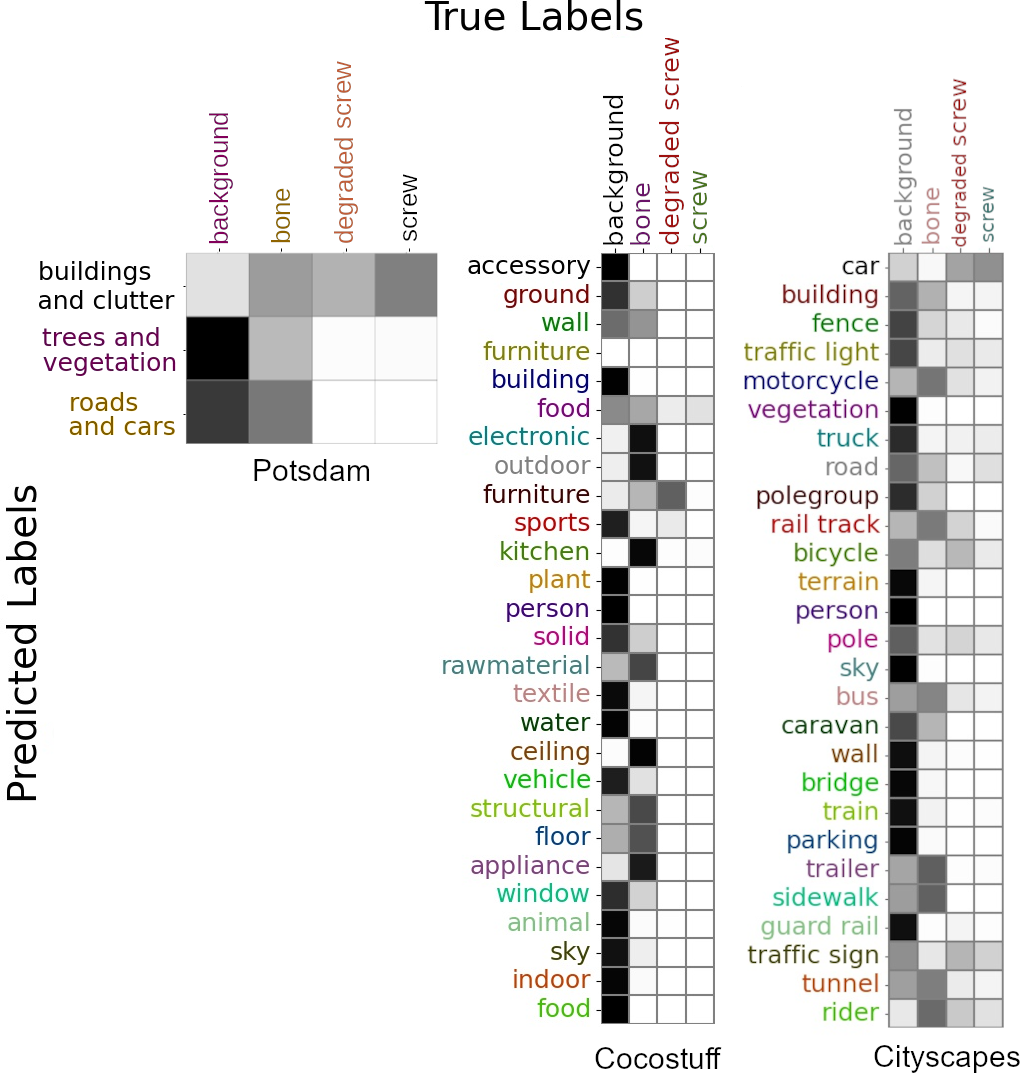
\includegraphics[width=\textwidth]{pictures/experiment_1/all_raw-cleaned_correlation_matrices}\\
    \caption[Correlation of Predicted Clusters to Labels]{Correlation matrix of ground truth labels and predicted clusters made with the three pre-trained models for the screws test set. Rows indicate predicted clusters, columns ground truth labels. \\ Ground truth label color indicates mapped model label. Dark color in the fields indicates a higher correlation coefficient than lighter color. Values are normed by row.}
    \label{fig:correlation-matrix-pretrained}
\end{figure}

\begin{figure}[!htb]
    \centering
    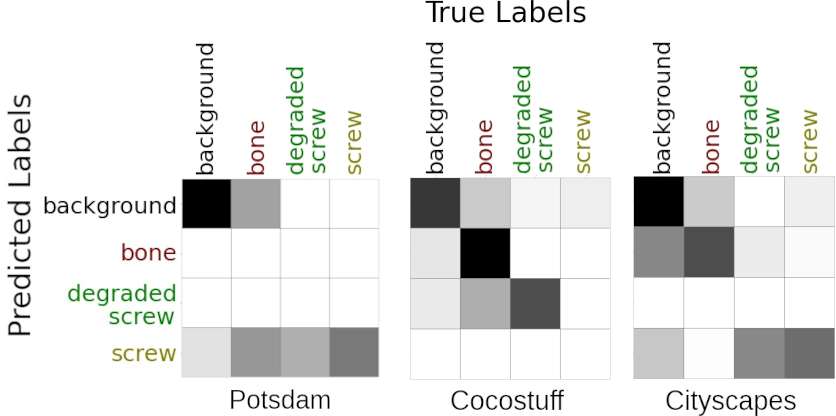
\includegraphics[width=0.9\textwidth]{pictures/experiment_1/all-combined_correlation_matrices}\\
    \caption[Correlation of Combined Clusters to Labels]{Correlation matrix of ground truth labels and merged predicted clusters made with the three pre-trained models for the screws test set. Rows indicate merged clusters, columns ground truth labels. Ground truth label color indicates mapped model label. Darker color in the fields indicates a higher correlation coefficient than lighter color. Values are normed by row. An exact model would be signified by a dark diagonal. Values are normed by row.}
    \label{fig:correlation-matrix-pretrained-combined}
\end{figure}

% Cocostuff
%model cluster - label assignment: 0: accessory, 1: ground, 2: wall, 3: furniture, 4: building, 5: food, 6: electronic, 7: outdoor, 8: furniture, 9: sports, 10: kitchen, 11: plant, 12: person, 13: solid, 14: rawmaterial, 15: textile, 16: water, 17: ceiling, 18: vehicle, 19: structural, 20: floor, 21: appliance, 22: window, 23: animal, 24: sky, 25: indoor, 26: food
% screws cluster to labels assignment: background = accessory, bone = food(1), degraded screw = sports, screw = kitchen
%cluster to label mapping
With the COCO-Stuff model, mapping single clusters to the ground truth labels via Hungarian matching found the following label assignments: the \formatLabel{accessory} cluster mapped to \formatLabel{background}, \formatLabel{food} (first occurrence) to \formatLabel{bone}, \formatLabel{sports} to \formatLabel{degraded screw} and \formatLabel{kitchen} to \formatLabel{screw}.
However, as seen in the correlation matrix (\autoref{fig:correlation-matrix-pretrained}), often multiple other categories were fully (or mostly) encompassed in one of the ground truth labels.
For example, the ground truth label \formatLabel{background} included most pixels belonging to \formatLabel{accessory, ground, wall, building, sport, plant, person, solid, textile, water, vehicle, window, animal, sky, indoor}, and the second \formatLabel{food} cluster;
the \formatLabel{bone} label included large parts of \formatLabel{vehicle, electronic, outdoor, kitchen, raw material, ceiling, structural, floor} and \formatLabel{appliance}.
The ground truth label \formatLabel{degraded screw} contained most \formatLabel{furniture} pixels, but did not correlate much with \formatLabel{sports}, to which it was mapped with Hungarian matching.
The correlation of \formatLabel{screw} was very weak for all clusters.
%combined clusters
When clusters were combined according to their most likely ground truth match (according to correlation value), three labels were reproduced: \formatLabel{background} (\gls{iou} of 0.69), \formatLabel{bone} (\gls{iou} of 0.37), and \formatLabel{degraded screw} (\gls{iou} 0.00).
However, mostly background was predicted, as seen in~\autoref{fig:pretrained-predictions}.
\begin{figure}[!htb]
    \centering
    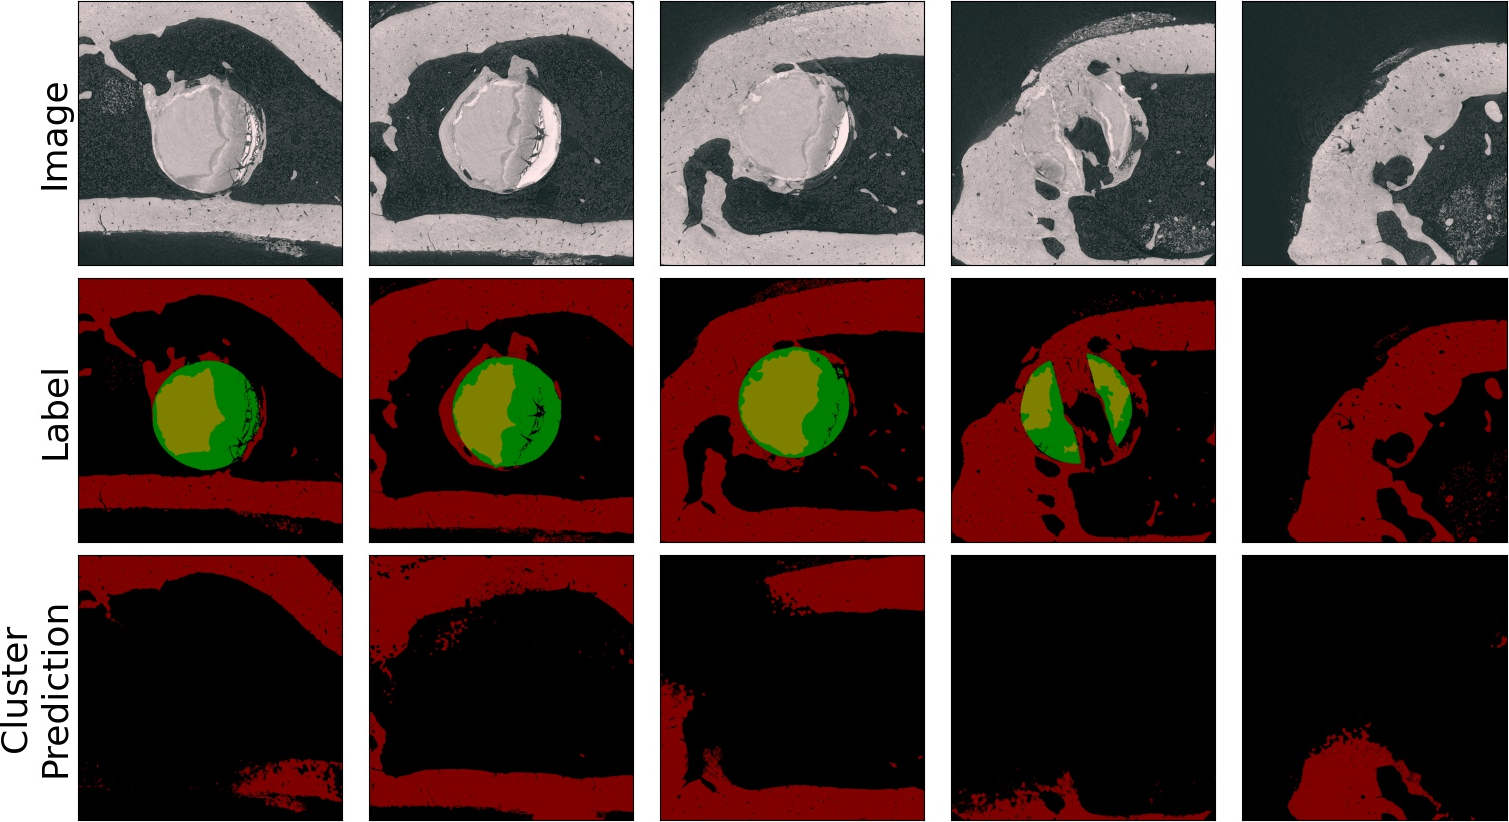
\includegraphics[width=0.95\textwidth]{pictures/experiment_1/cocostuff-combined_example_predictions_0_small}\\
    \caption[Additional Combined Clusters of COCO-Stuff]{Visualisation of image, ground truth, and clusters combined by their most likely match to ground truth labels for COCO-Stuff predictions. All shown slices belong to the second half of volume 113729HQMg5 and are ordered according to spatial location in the volume. Every 100th slice is shown.}
    \label{fig:more-cocostuff-predictions}
\end{figure}

% manual clusters
When looking at the predictions in~\autoref{fig:pretrained-predictions}, the big purple \formatLabel{food} cluster stands out, since it seems to neatly encompass the full bone (including bone marrow and screw) on some slices (on other predictions it encompasses only bone marrow), see~\autoref{fig:more-cocostuff-predictions}.
It was decided to manually assign this cluster to \formatLabel{bone}, since it mostly included bone and also bone marrow. 
The high correlation value with \formatLabel{background} was calculated because in the ground truth, bone marrow was mostly assigned to \formatLabel{background} and not \formatLabel{bone}, since segmentation was based on a thresholding method.
With this manual assignment, predictions of \formatLabel{bone} improved slightly (from \gls{miou} of 0.35 to 0.44), while \gls{iou} of \formatLabel{background} slightly decreased from 0.69 to 0.63.
The \formatLabel{degraded screw} label did not change at all, as was to be expected, since no pixel was removed or added to this label.
A visualisation of this manual assignment in comparison to assignment by correlation value can be found in~\autoref{fig:cocostuff-compare-manualcombine-predictions}.
\begin{figure}[!htb]
    \centering
    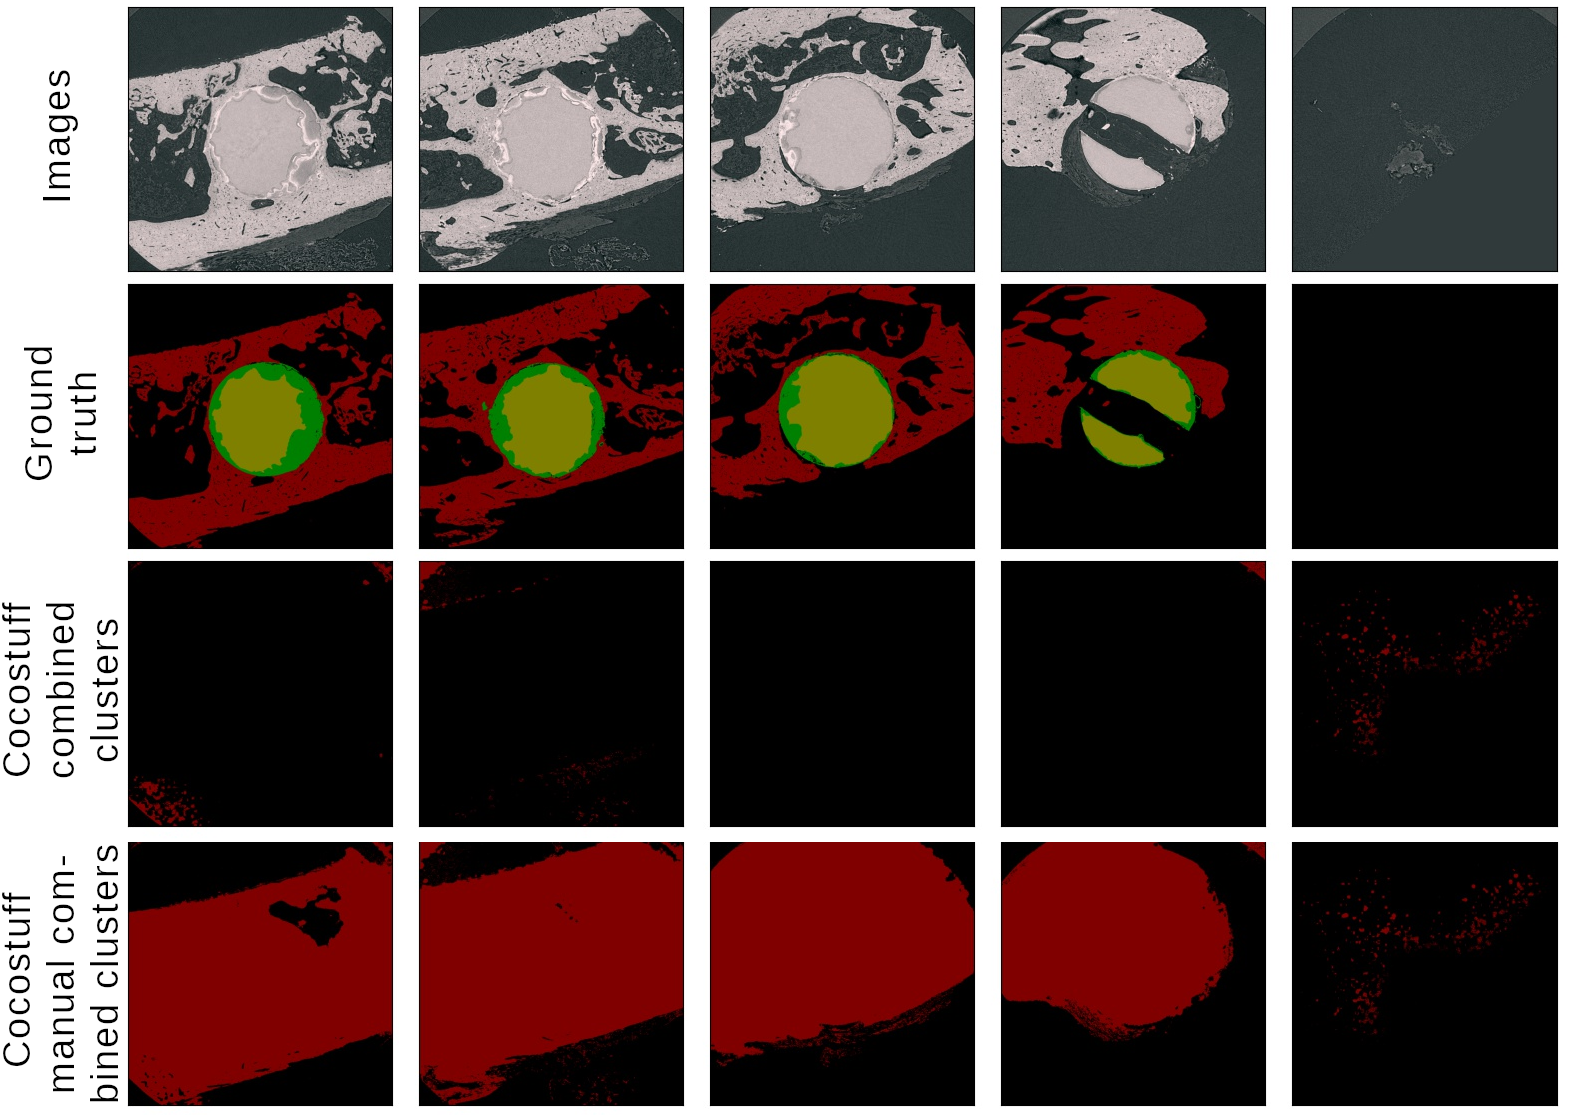
\includegraphics[width=\textwidth]{pictures/experiment_1/cocostuff-compare-manual-combined_example_predictions_2}\\
    \caption[Manually Combined Clusters of COCO-Stuff]{Image, ground truth, and manually combined clusters of predictions made with the COCO-Stuff model. All shown slices belong to the second half of volume syn009HQ (which was neither part of train nor validation set) and are ordered according to spatial location in the volume. Every 100th slice is shown.}
    \label{fig:cocostuff-compare-manualcombine-predictions}
\end{figure}

% Cityscapes
%model cluster to label assignment:  0: car, 1: building, 2: fence, 3: traffic light, 4: motorcycle, 5: vegetation, 6: truck, 7: road, 8: polegroup, 9: rail track, 10: bicycle, 11: terrain, 12: person, 13: pole, 14: sky, 15: bus, 16: caravan, 17: wall, 18: bridge, 19: train, 20: parking, 21: trailer, 22: sidewalk, 23: guard rail, 24: traffic sign, 25: tunnel, 26: rider
% road = background, bus = bone, rail track = degraded screw, truck = screw
%cluster to label mapping
With the Cityscapes model, mapping single clusters to the ground truth labels with Hungarian matching yields the following assignments: \formatLabel{road} mapped to \formatLabel{background}, \formatLabel{bus} to \formatLabel{bone}, \formatLabel{rail track} to \formatLabel{degraded screw} and \formatLabel{truck} to \formatLabel{screw}.
Again, these mappings were not the only candidates as seen in~\autoref{fig:correlation-matrix-pretrained-combined}.
Large parts of \formatLabel{building, fence, traffic light, vegetation, truck, polegroup, terrain, person, pole, sky, caravan, wall bridge, train, parking}, and \formatLabel{guard rail} also correlated with \formatLabel{background}, while large parts of \formatLabel{motorcycle, rail track, bus, trailer, sidewalk, tunnel}, and \formatLabel{rider} also correlated strongly with \formatLabel{bone}.
On the other hand, the correlation of \formatLabel{rail track} to the \formatLabel{degraded screw} label (which it was assigned to with Hungarian matching) was also very weak, while the correlation of \formatLabel{furniture} is higher.
% combined clusters
Combining all clusters by their most likely ground truth mapping produced good predictions of \formatLabel{background} (\gls{iou} of 0.63), intermediate predictions of \formatLabel{bone} (\gls{iou} 0.37), and basically no predictions of \formatLabel{degraded screw} and \formatLabel{screw}.
This was also reflected in the correlation matrix (\autoref{fig:correlation-matrix-pretrained-combined}), where only \formatLabel{background} and \formatLabel{bone} correlated at a higher rate.

\begin{figure}[!htb]
    \centering
    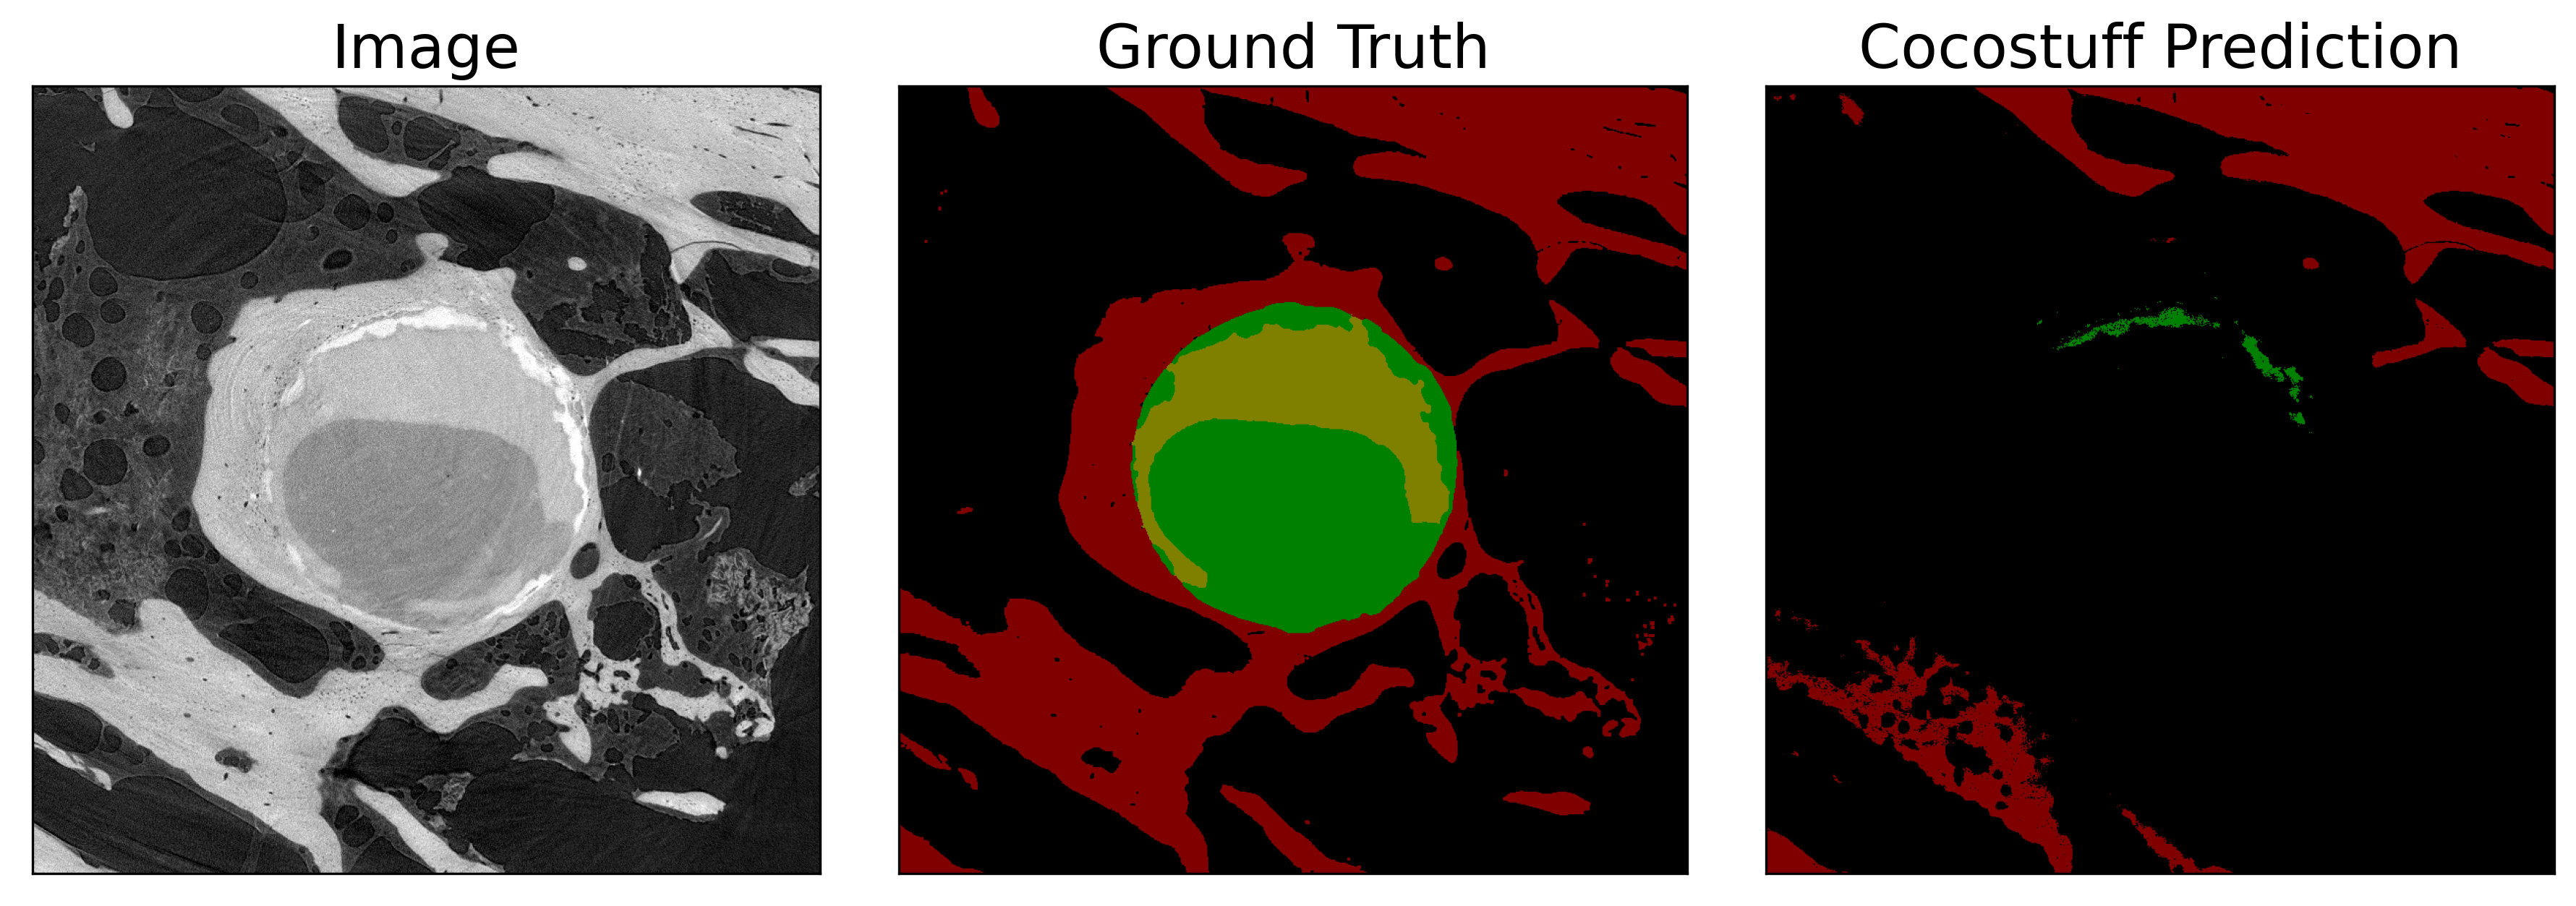
\includegraphics[width=\textwidth]{pictures/experiment_1/113734HQMg5_direction0_slice0670_cocostuff_prediction_with_degraded_screw_prediction}\\
    \caption[Degraded Screw Prediction of COCO-Stuff]{Image, ground truth and prediction with the COCO-Stuff model of slice 670 from volume 113734HQMg5, to show size and location of \formatLabel{degraded screw} predictions. This slice has the biggest area of the \formatLabel{degraded screw} prediction (2328 pixels), which is located at the edge of the ground truth label. Most other slices only contain very few pixels.}
    \label{fig:cocostuff-degradedscrew-example}
\end{figure}

Generally, there were only a few pixels identified as \formatLabel{screw}.
Only 267 (often not concurrent slices) of the 3000~slices test set contained \formatLabel{screw} pixels.
Additionally, these patches were very small, and only comprise few pixels each, which were aligned around the edges of the ground truth label, as seen in~\autoref{fig:cocostuff-degradedscrew-example}.
Thus overall-correlation of the few pixels, that were found, was quite high, as seen in \autoref{fig:correlation-matrix-pretrained-combined}, meaning there were few false positives.
However, most real \formatLabel{screw} pixels are identified (wrongly) as \formatLabel{background}.
Overall, the \gls{miou} of the combined clusters for the Cityscapes model was~0.26.
% contain the floats in section
\afterpage{\FloatBarrier}

% wrap up for all three
None of the three models was able to differentiate all ground truth labels.
At least one label was missing in each.
Additionally, the predictions were often not very good.
All three models reached \gls{iou} values between 0.6 and 0.7 for \formatLabel{background}, around 0.3 for \formatLabel{bone} (if it was predicted at all) and 0.36 (Potsdam) or nearly 0 (Cityscapes) for \formatLabel{screw}.
\formatLabel{Degraded screw} was only predicted with COCO-Stuff, but the \gls{iou} was nearly 0 there, too.


\subsubsection{Experiment 2: Train on Scientific Data Set}\label{subsubsec:results-experiment2res}

% runtimes and batch sizes
Training was done on different configurations with different image resolutions and thus, batch sizes.
Batch size of the base case was 8, for the 200~px random cropped regime it could be increased to 16, and for the 96~px random cropped regime it could be doubled to 32 again.
This means, runtimes varied between 1.5~hours and more than a day, depending on the configuration.
An overview on the runtimes can be found in ~\autoref{tab:runtimes}.
Because the batch size varied, the number of steps in one epoch\footnote{One epoch is a full run through all training examples, and steps are defined as one run through a batch. For multi-GPU-training a step is one run through a batch on all GPUs.} also varied, but due to different image sizes, the number of seen pixels are the same between steps.
For example, due to the four times higher batch size (and 5.2~times smaller image size), the model trained on the 96~px random cropped data set was trained on four times more training images per step, but only 0.8~times the number of pixels in comparison to the base case.
Similar proportions are true for the 200~px random cropped model, where the batch size was half the size in comparison to the base case, and the image size was 0.4~times smaller.\footnote{That means, the two random cropped regimes were trained on nearly the same pixel numbers at each step.}

\begin{table}[!bht]
    \caption[Best Models Accuracy per Fold]{Best models accuracy (proportion of correctly classified pixels) per fold. Models are identified by cropping regime, resolution, and fold.\textsuperscript{*} For each model the accuracy on the validation set and [step] at which it occurred is given. Additionally, mean and standard deviation of accuracy over folds is reported. Values are rounded to the second decimal. Note, that step numbers between models do not correspond, and folds between leave-one-out (LOO) and all others differ.}
    \label{tab:accuracy-step-by-fold}
    \makegapedcells      % in makecell
    \centering
    \begin{tabular}{|>{\bfseries}c|>{\raggedright\arraybackslash}p{0.11\textwidth}|>{\raggedright\arraybackslash}p{0.11\textwidth}|>{\raggedright\arraybackslash}p{0.115\textwidth}|>{\raggedright\arraybackslash}p{0.11\textwidth}|>{\raggedright\arraybackslash}p{0.11\textwidth}||r|}
        \hline
        \makecell[cb]{} & \makecell[c]{\textbf{Fold 0}} & \makecell[c]{\textbf{Fold 1}} &
        \makecell[c]{\textbf{Fold 2}} & \makecell[c]{\textbf{{Fold 3}}} & \makecell[c]{\textbf{Fold 4}} & \textbf{mean}\\ \hline
        % base-case
        \makecell[c]{\hspace{1mm}base\\case} & \makecell[r]{0.71 \\\emph{\small[1,249]}} & \makecell[r]{0.71 \\\emph{\small[2,718]}} & \makecell[r]{0.65 \\\emph{\small[499]}} & \makecell[r]{0.70 \\\emph{\small[499]}} & \makecell[r]{0.73 \\ \emph{\small[3,124]}} & \makecell[r]{0.70\\ ± 0.03} \\ \hline
        % random 200px  
        \makecell{random\\cropped\\200~px} & \makecell[r]{0.63 \\\emph{\small [1,359]}}	&	\makecell[r]{0.64 \\\emph{\small [1,359]}} & \makecell[r]{ 0.66 \\ \emph{\small [1,359]}} & \makecell[r]{ 0.67 \\\hspace{-2.2mm}\emph{\small [11,679]}} & \makecell[r]{ 0.58 \\ \emph{\small [249]}} & \makecell[r]{0.64\\ ± 0.04}\\ \hline
        % radom 96px  
        \makecell{random\\cropped\\96~px} & \makecell[r]{0.76 \\ \emph{\small [1,539]}} & \makecell[r]{0.61 \\ \emph{\small [8,419]}} & \makecell[r]{ 0.57 \\ \emph{\small [249]}} & \makecell[r]{0.63 \\\emph{\small [4,549]}} & \makecell[r]{0.59 \\ \emph{\small [249]}} & \makecell[r]{0.63\\± 0.08} \\ \hline
        % LOO
        & \makecell[c]{\textbf{LOO 0}} & \makecell[c]{\textbf{LOO 1}} &
        \makecell[c]{\textbf{LOO 2}} & \makecell[c]{\textbf{{LOO 3}}} & \makecell[c]{\textbf{LOO 4}} & \textbf{mean}\\ \hline
        \makecell{leave-\\one-\\out} & \makecell[r]{0.69 \\ \emph{\small [6,845]}} & \makecell[r]{0.66 \\ \emph{\small [7,595]}} & \makecell[r]{ 0.83 \\ \emph{\small [29,447]}} & \makecell[r]{0.68 \\\emph{\small [1,999]}} & \makecell[r]{0.68 \\ \emph{\small [8,877]}} & \makecell[r]{0.71\\± 0.07} \\ \hline
    \end{tabular}
    \raggedright
    \\ \small\textsuperscript{*}Extra cluster regimes are not reported here, since accuracy is misleading in these.
\end{table}

\begin{table}[p]
    \caption[Best Models mIoU per Fold]{Best models mIoU per fold. Models are identified by cropping regime, resolution, and fold.\textsuperscript{*} For each model the mIoU on the validation set and standard deviation is given. Additionally, mean and standard deviation of mIoU over folds is reported. Values are rounded to the second decimal. Note, that folds between leave-one-out (LOO) cross-validation and all others differ.}
    \label{tab:miou-by-fold}
    \makegapedcells      % in makecell
    \centering
    \begin{tabular}{|>{\bfseries}c|>{\raggedright\arraybackslash}p{0.11\textwidth}|>{\raggedright\arraybackslash}p{0.11\textwidth}|>{\raggedright\arraybackslash}p{0.115\textwidth}|>{\raggedright\arraybackslash}p{0.11\textwidth}|>{\raggedright\arraybackslash}p{0.11\textwidth}||r|}
        \hline
        \makecell[cb]{} & \makecell[c]{\textbf{Fold 0}} & \makecell[c]{\textbf{Fold 1}} &
        \makecell[c]{\textbf{Fold 2}} & \makecell[c]{\textbf{{Fold 3}}} & \makecell[c]{\textbf{Fold 4}} & \textbf{mean}\\ \hline
        % base-case
        \makecell[c]{\hspace{1mm}base\\case} & \makecell[r]{0.49 \\ ± 0.35} & \makecell[r]{0.49 \\ ± 0.34} & \makecell[r]{0.43 \\± 0.29} & \makecell[r]{0.45 \\±0.30} & \makecell[r]{0.50 \\ ± 0.34} & \makecell[r]{0.47\\ ± 0.03} \\ \hline
        % random 200px  
        \makecell{random\\cropped\\200~px} & \makecell[r]{0.44 \\± 0.33}	&	\makecell[r]{0.48 \\± 0.35} & \makecell[r]{ 0.44 \\ ± 0.30} & \makecell[r]{ 0.44 \\± 0.32} & \makecell[r]{ 0.39 \\ 27} & \makecell[r]{0.44\\ ± 0.03}\\ \hline
        % radom 96px  
        \makecell{random\\cropped\\96~px} & \makecell[r]{0.57 \\ ± 0.30} & \makecell[r]{0.39 \\ ± 0.28} & \makecell[r]{ 0.38 \\ ± 0.20} & \makecell[r]{0.46 \\± 0.33} & \makecell[r]{0.41 \\ ± 0.21} & \makecell[r]{0.44\\± 0.08} \\ \hline
        & \makecell[c]{\textbf{LOO 0}} & \makecell[c]{\textbf{LOO 1}} &
        \makecell[c]{\textbf{LOO 2}} & \makecell[c]{\textbf{{LOO 3}}} & \makecell[c]{\textbf{LOO 4}} & \textbf{mean}\\ \hline
        \makecell{leave-\\one-\\out} & \makecell[r]{0.54 \\ ± 0.33} & \makecell[r]{0.41 \\ ± 0.29} & \makecell[r]{ 0.61 \\ ± 0.39} & \makecell[r]{0.47 \\± 0.32} & \makecell[r]{0.47 \\ ± 0.34} & \makecell[r]{0.50\\± 0.08} \\ \hline
    \end{tabular}
%Extra cluster regimes are not reported here, since \gls{miou} is misleading in these. 
    \caption[Best Models IoU per Label]{Best models IoU per label. Models are identified by cropping regime and resolution or cross-validation scheme.\textsuperscript{*} For each model, IoU and standard deviation of IoU for each label (as well as mean over all labels and standard deviation between labels) on the validation set over the cross-validation is given. Values are rounded to the second decimal.}
    \label{tab:miou-by-label}
    \makegapedcells      % in makecell
    \centering
    \begin{tabular}{|>{\bfseries}c|>{\raggedright\arraybackslash}p{0.13\textwidth}|>{\raggedright\arraybackslash}p{0.13\textwidth}|>{\raggedright\arraybackslash}p{0.15\textwidth}|>{\raggedright\arraybackslash}p{0.13\textwidth}||>{\raggedright\arraybackslash}p{0.1\textwidth}|}
        \hline
        & \makecell[c]{\textbf{\formatLabel{back-}} \\ \textbf{\formatLabel{ground}}} & \makecell[c]{\textbf{\formatLabel{bone}}} &
        % else we get an ugly linebreak in cell
        \makecell[c]{\hspace{-0.5mm}\textbf{\formatLabel{degraded}} \\ \textbf{\formatLabel{screw}}} & \makecell[c]{\textbf{\formatLabel{screw}}} & \makecell[c]{\textbf{mean}} \\ \hline
        %base-case
        \makecell{base case} & \makecell[r]{0.59 \\± 0.04} & \makecell[r]{0.69 \\± 0.11} & \makecell[r]{0.00 \\± 0.00} & \makecell[r]{0.61 \\± 0.03} & \makecell[r]{0.47\\± 0.32}  \\ \hline
        % random 200px  
        \makecell{random\\cropped\\200~px} & \makecell[r]{0.48 \\± 0.04}	&	\makecell[r]{0.62 \\± 0.11} & \makecell[r]{0.00 \\± 0.00} & \makecell[r]{0.66 \\± 0.09} & \makecell[r]{0.44\\± 0.30}	 \\ \hline
        % radom 96px  
        \makecell{random\\cropped\\96~px} & \makecell[r]{0.52 \\± 0.10} & \makecell[r]{0.61 \\± 0.10} & \makecell[r]{0.06 \\± 0.05} & \makecell[r]{0.57 \\± 0.13} & \makecell[r]{0.44\\± 0.26} \\ \hline
        % LOO
        \makecell{leave-one-\\out} & \makecell[r]{0.61 \\± 0.12}	&	\makecell[r]{0.74 \\± 0.08} & \makecell[r]{0.02 \\± 0.03} & \makecell[r]{0.62 \\± 0.13} & \makecell[r]{0.50\\± 0.32}	 \\ \hline
    \end{tabular}
    \raggedright
    \\ \small\textsuperscript{*}Extra cluster regimes are not reported here, since \gls{iou} is misleading in these.
\end{table}

%weights
Since cropping changes the images used for training, the parameter tuning needed to be done separately for each training.
Only the base case and the extra cluster trainings could be run with the same parameters, since there were no differences between the training data (only differences in configurations to allow for extra clusters).
An overview of the parameters can be found in the appendix in ~\autoref{tab:training-parameters}.

% base case
The base case was trained on the five-cropped data set, as explained before.
% explain images
Example predictions of the different base case folds can be found in~\autoref{fig:example-predictions-folds-base-case}.
Predictions between folds differed slightly, especially in slices stemming from the edges of the volumes (see last image in~\autoref{fig:example-predictions-folds-base-case}).
Additionally, predictions of areas outside the sample were often assigned to different labels, as seen in the second to fourth images in~\autoref{fig:example-predictions-folds-base-case}.
%explain mIoU
As seen in \autoref{tab:miou-by-fold}, \gls{miou} varied between folds and peaked around 0.50 in the different folds.
The course of the accuracy is basically the same, but shifted upwards, as seen in~\autoref{fig:accuracy-per-fold}, thus in the following, the focus is laid on the \gls{miou}.
In all five folds, this peak (the best model) was reached relatively early during training, between the~500th and~3,200th step~(\autoref{tab:accuracy-step-by-fold}).
Afterwards, \gls{miou} decreased to around~0.35 to~0.40.
As seen in \autoref{fig:miou-per-fold-label} and \autoref{tab:miou-by-label}, performance between the labels highly differed.
Label \formatLabel{bone} performed best (\gls{iou} in the folds was 0.69~±~0.11), followed by \formatLabel{screw} (\gls{iou} of 0.61~±~0.03) and \formatLabel{background} (\gls{iou} of 0.59~±~0.04), while \formatLabel{degraded screw} could not be detected at all (\gls{iou} of 0.00~±~0.00).
This difference in performance can also be seen in the accuracy values of the folds (see~\autoref{tab:accuracy-step-by-fold}), which are generally higher than the \gls{miou}, but similarly distributed, as seen in~\autoref{fig:accuracy-mIoU-boxplots}.
\afterpage{\FloatBarrier}
% comparison to random cropped
Trainings on the random cropped data sets did not differ much from the five-cropped base case in regard to \gls{miou} (which was 0.44~for both resolutions used), but there were differences in \gls{iou} between folds and labels (as seen in~\autoref{tab:miou-by-label},~\autoref{fig:miou-per-fold},~and ~\autoref{fig:miou-per-fold-label}).
Additionally, it can be seen in~\autoref{fig:example-predictions-fold2} that differences in predictions between the cropping regimes occurred on similar occasions (on slices at the edge of the 3D volumes, and outside the specimen) as differences between folds.
Divergence of \gls{miou} between folds was very pronounced in the 96~px random cropped regime, where fold~0 performed a lot better than all other folds (nearly two standard deviations difference in \gls{miou}).
For the training made on the 200~px random cropped data set, the best models were, again, reached early during training, between step 249 and 1,359.\footnote{Since image size and batch sizes differed between base case and random cropped trainings, this step number does not correspond to the base case in terms of training examples or pixels seen.
The 200~px random cropped regime saw two times more, the 96~px random cropped regime four times more training examples per step, but they both saw only 0.8 times the pixel number of the base case.}


\begin{figure}[p]
    \centering  %trim={<left> <lower> <right> <upper>}
    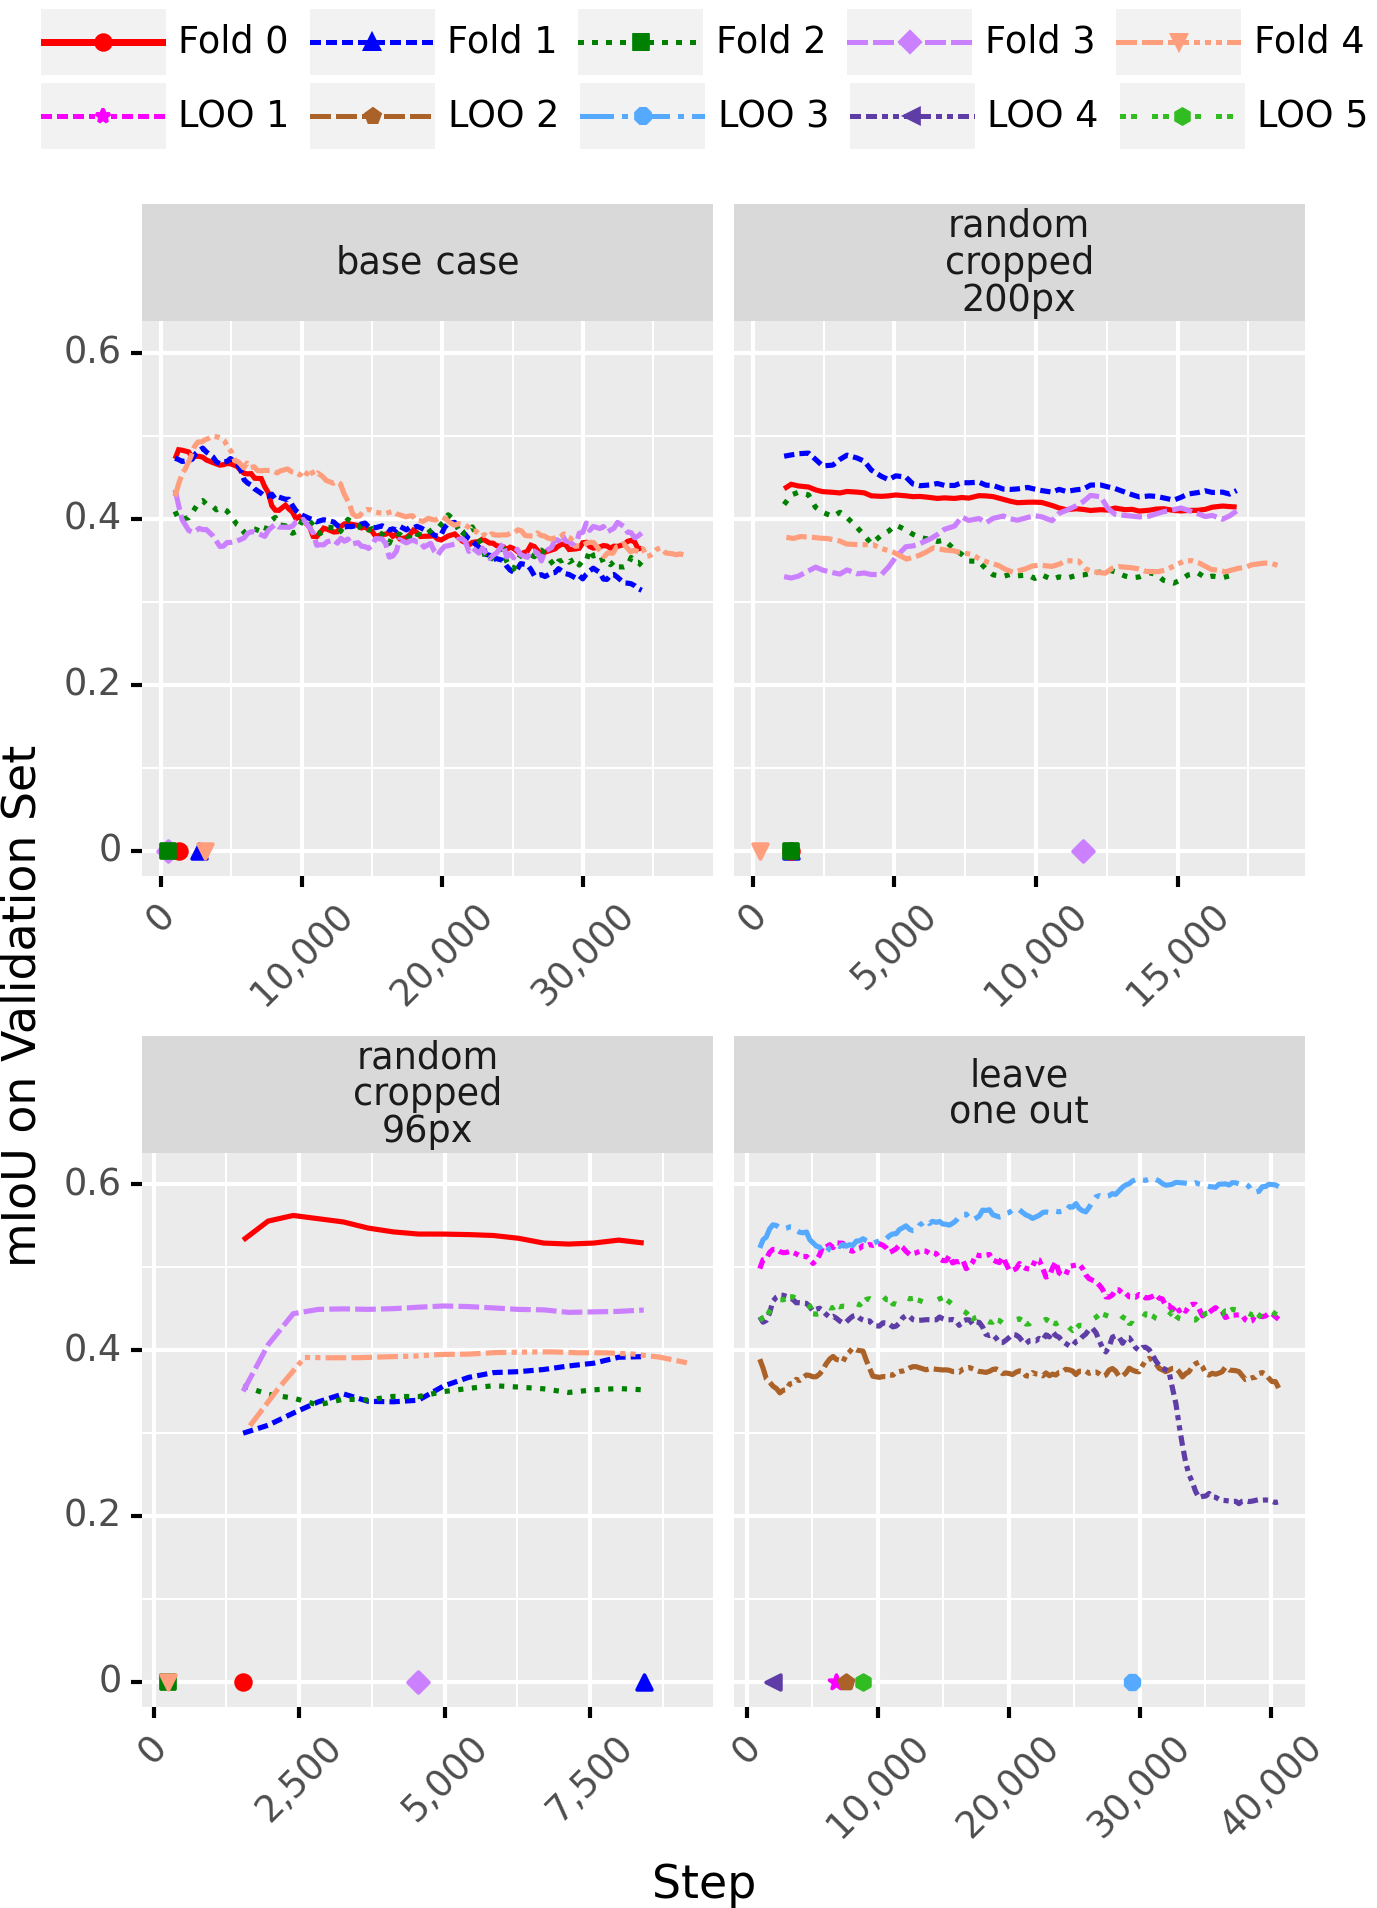
\includegraphics[width=\textwidth]{pictures/experiment_2/mIoU_base-case_final_base-case_loo_random_cropped_final_random_cropped_res96_final}\\
    \caption[Fold-wise Development of mIoU]{Fold-wise development of mIoU. For each cross-validation, the moving average (over three data points) of the mIoU per fold is displayed. So the first three data points are not depicted in the plots. Additionally, on the x-axis the step number of the best overall model per fold (in terms of mIoU) is marked.\\}  % to have only this figure on page
    \label{fig:miou-per-fold}
\end{figure}

\begin{figure}[p]
    \centering
    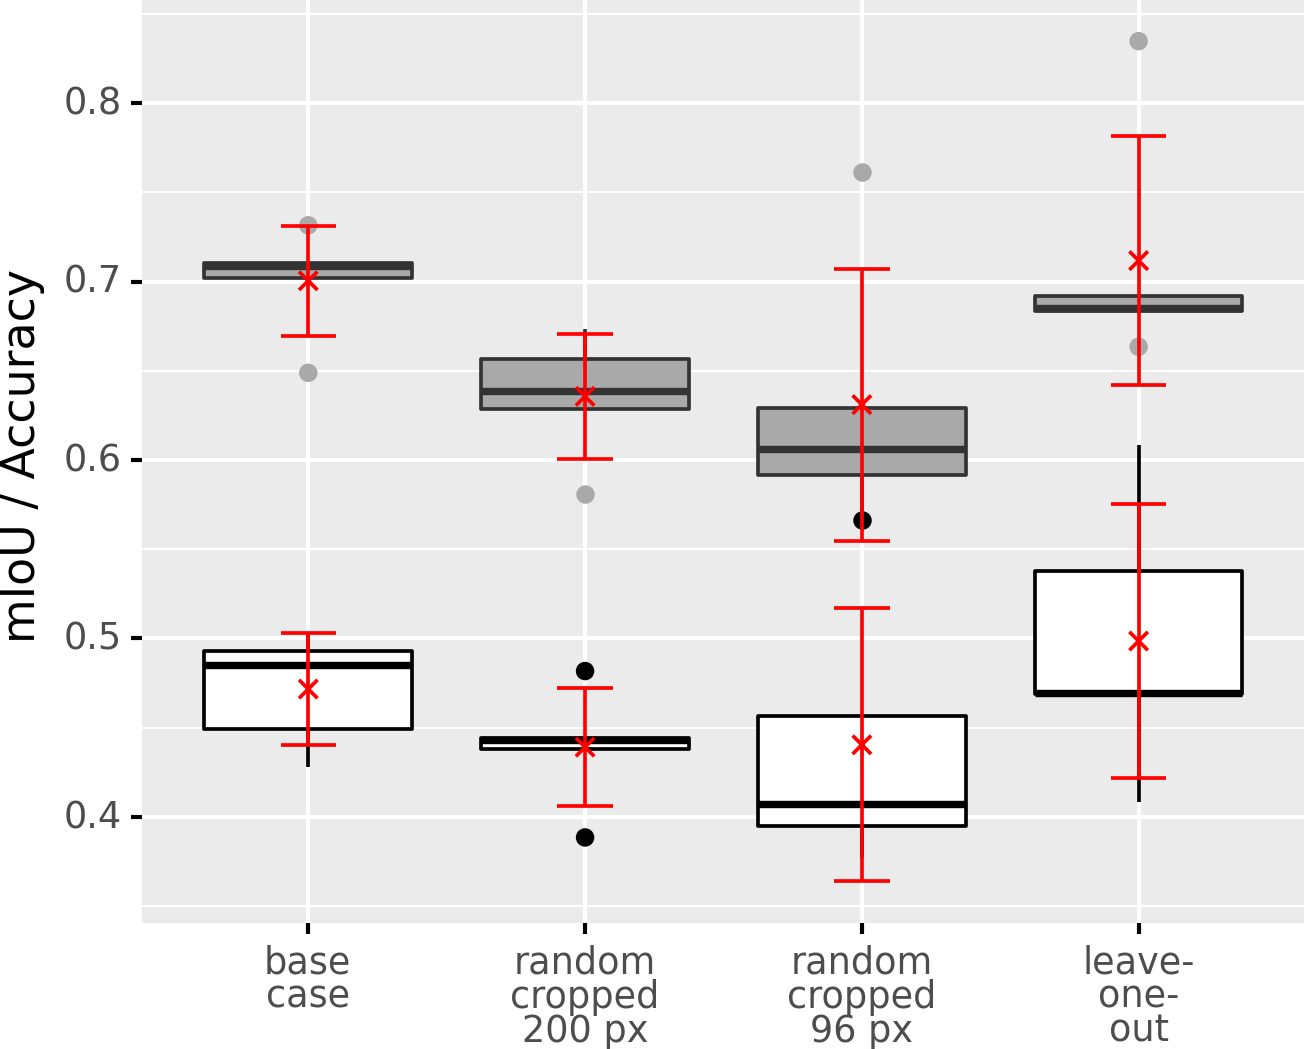
\includegraphics[width=0.8\textwidth]{pictures/experiment_2/compare_all_model_stats_mIoU_accuracy}\\
    \caption[Boxplots of mIoU and Accuracy for Best Models]{Boxplots of the accuracy (grey) and mIoU (white) for all folds of a configuration. Boxplots indicate the median as solid line, the hinges indicate the inter-quartile range, the whiskers correspond to 1.5 inter-quartile range, and outliers are indicated as points. Additionally, marked in red are mean and standard deviation.\\}
    %box=50% of data (Inter-Quartile Range (IQR)), line=median, whisker=1.5 IQR, Outliers.
    \label{fig:accuracy-mIoU-boxplots}
    \centering
    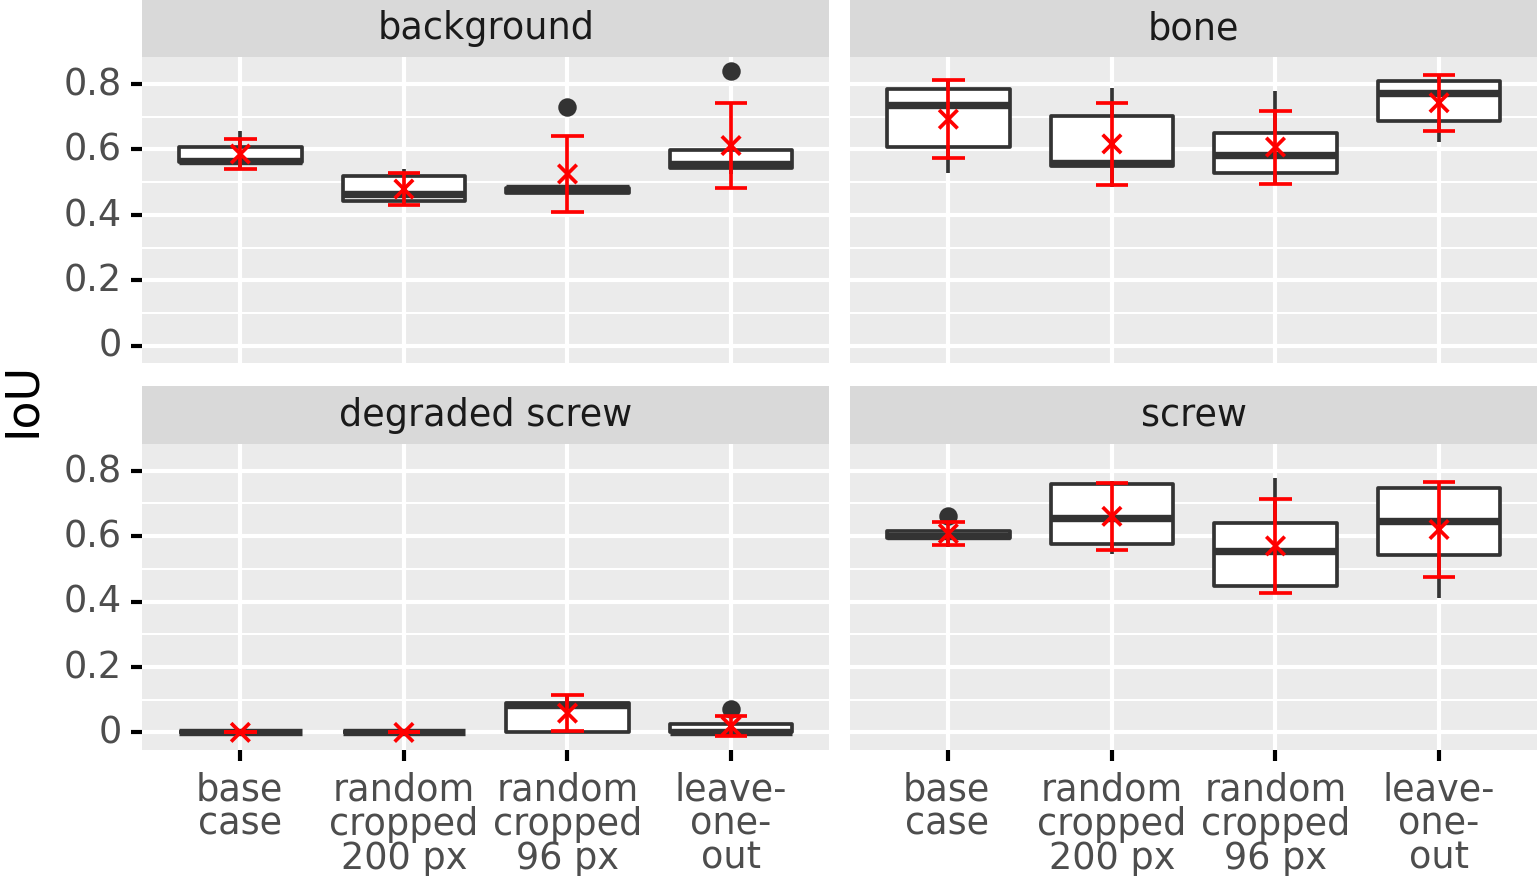
\includegraphics[width=\textwidth]{pictures/experiment_2/compare_all_model_stats_labelwise}\\
    \caption[Labelwise Boxplots of IoU for Best Models]{Boxplots of the IoU for all folds of a configuration. Boxplots indicate the median as solid line, the hinges indicate the inter-quartile range, the whiskers correspond to 1.5 inter-quartile range, and outliers are shown. Additionally, marked in red are mean and standard deviation.}
    %box=50% of data (Inter-Quartile Range (IQR)), line=median, whisker=1.5 IQR, Outliers.
    \label{fig:mIoU-boxplots-labelwise}
\end{figure}


% divergence of folds (and models)
In the random cropping regimes, the folds diverged too\footnote{Additional side-by-side plots of predictions between folds are found in the appendix in~\autoref{subsec:example-predictions-for-cropping-regimes}}, but visually predictions were more similar, as seen in the example predictions of different folds for same image in~\autoref{fig:example-predictions-fold2}.
As seen in \autoref{tab:miou-by-fold}, and visualised in \autoref{fig:accuracy-mIoU-boxplots} and~\ref{fig:mIoU-boxplots-labelwise}, divergence between folds was the same between 200~px random cropped regime and the base case (standard deviation of \gls{miou} between folds was~0.03), and higher in the 96~px random cropped regime, where the standard deviation nearly tripled (to ~0.08).
The standard deviation of \gls{iou} per label between the folds is 0.13~at worst, and 0.03~to~0.04 at best, on all models~(\autoref{tab:miou-by-label}).
Since \formatLabel{degraded screw} was not found in a relevant quantity in any model, the standard deviation is not meaningful for this label.
The divergence is highest for the label \formatLabel{bone} in all models (standard deviation of \gls{iou} of labels~0.10~to~0.11).
Overall, divergence on the 96~px random cropped model is higher in comparison to the other models.
In the label \formatLabel{background}, the standard deviation more than doubled, in \formatLabel{bone}, the standard deviation was more than three times higher than in the base case, while the standard deviation of \formatLabel{bone} stayed nearly the same.

% LOO
A leave-one-out cross-validation was done to investigate this divergence, as especially with small data sets training on more data is often beneficial.
As seen in~\autoref{fig:miou-per-fold}, the leave-one out cross-validation generally behaves more stable than the base case.
The decrease in \gls{iou} is not as pronounced as with five-cold cross validation.
Generally, there was a slight increase in \gls{iou} of the labels (0.02~to~0.05~points \gls{iou}) and also in \gls{miou} (0.03~points), but also often the variability between labels of the same fold increased.
Standard deviation between folds was three to four times higher in most labels, compared to the base case, but the standard deviation of the \gls{miou} was the same~(0.32), and standard deviation of the \gls{miou} nearly tripled to~0.08 in comparison to the base case.
As not all folds of the leave-one-out cross-validation were trained, this metric must be considered with caution, as the other nine folds might still change this significantly.
%LOO: predictions
When considering the predictions of the leave-one-out folds (see~\autoref{fig:example-predictions-folds-loo}), they seem visually very similar to the base case predictions.
Predictions of slices from the edge of the volume and regions outside the sample often are poor, and often the \formatLabel{degraded screw} label is mapped there, as it was also the case in the five-fold cross-validation.

%extra clusters
To further investigate the poor performance of the \formatLabel{degraded screw} label, additional trainings were done with overclustering to allow \gls{stego} to find more clusters than labels and map only the most promising candidates to the labels during validation.
However, as seen in the example predictions (\autoref{fig:example-predictions-fold2}), even with allowing 10~extra clusters, no cluster corresponding to the \formatLabel{degraded screw} label could be found\footnote{Since the evaluation of extra clusters is only done on pixels that were assigned to a ground truth label (not to extra clusters), \gls{miou} values will not be discussed, since they are misleading.}.
But the differentiation of bone and bone marrow, and tissue and sample background improves visibly.

Considering all trained models, even though there is some variability, the best models found are quite similar between folds, and also between different cropping regimes.
This is illustrated in~\autoref{fig:full-example-predictions-slice500}, where the same slice is predicted with each fold of each model.
In some models, areas outside the sample are mapped to different labels (often \formatLabel{degraded screw} or \formatLabel{screw}), but there is no obvious pattern regarding fold or cropping regime.
%All models do predict \formatLabel{screw} quite well, similarly for \formatLabel{bone} and \formatLabel{background}, while no model performs well on \formatLabel{degraded screw}.


\begin{figure}[p]
    \centering
    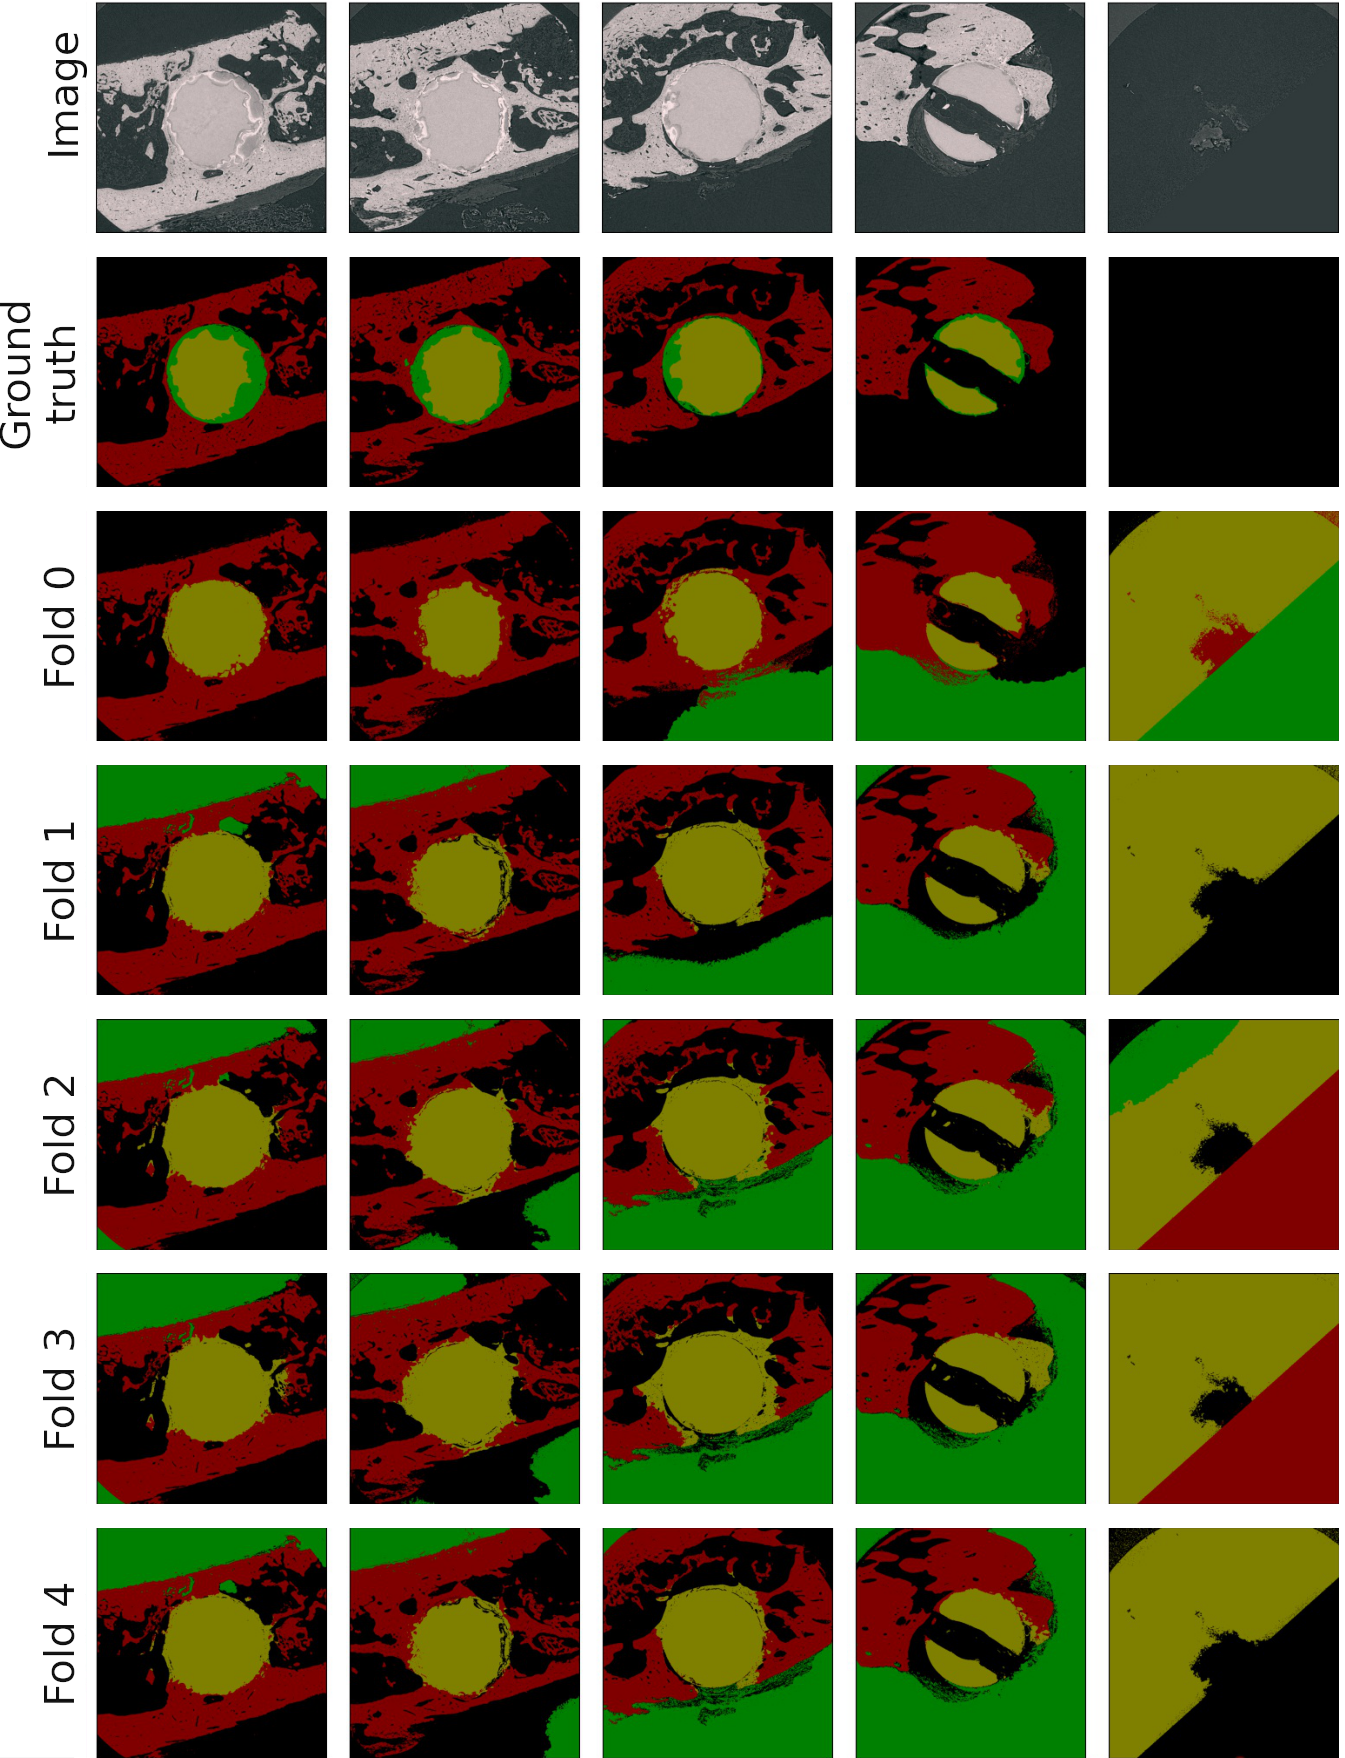
\includegraphics[width=\textwidth]{pictures/experiment_2/for_paper_base-case_final_example_predictions_2_all_folds}\\
    \caption[Foldwise Predictions of the Base Case]{Example predictions of the best models from different folds of the base case. All shown slices belong to the second half of volume syn009HQ (which was neither part of train nor validation set) and are ordered according to spatial location in the volume. Every 100th slice is shown.}
    \label{fig:example-predictions-folds-base-case}
\end{figure}


\begin{figure}[p]
    \centering
    %\vspace{1em}
    \includegraphics[width=\textwidth]{pictures/experiment_2/all_experiments_all_folds_example_predictions2_slice_500}\\
    \caption[Comparison of Predicitons for Same Slice]{Example predictions of the same slice for all best models (all folds). Not shown: leave-one-out cross-validation, since the folds do not correspond. Shown is slice 500 of volume syn009HQ (which was neither part of train nor validation set).}
    \label{fig:full-example-predictions-slice500}
\end{figure}


\begin{figure}[p]
    \centering
    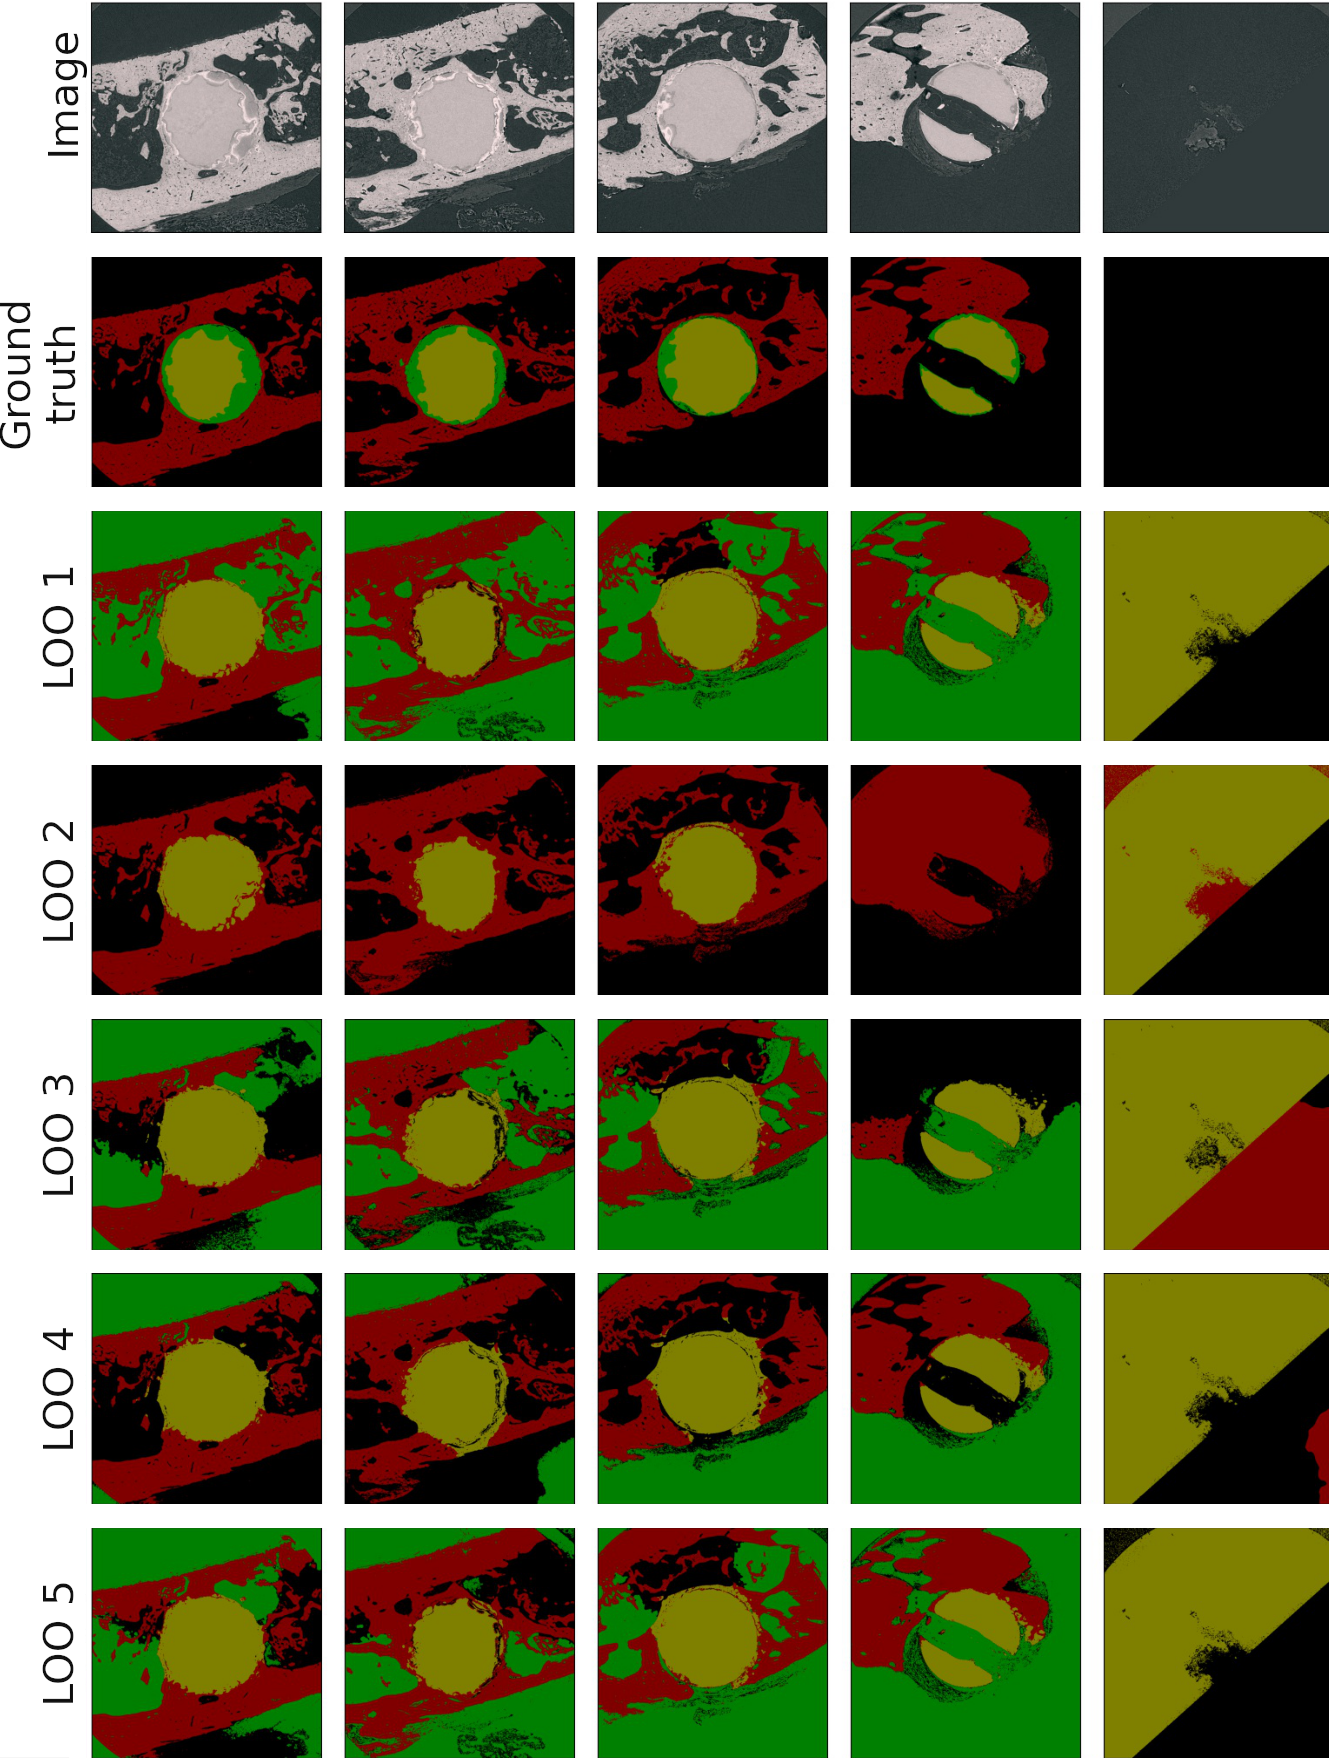
\includegraphics[width=\textwidth]{pictures/experiment_2/for_paper_base-case_LOO_example_predictions_2_all_folds}\\
    \caption[Predictions for Different Leave-one-out Folds]{Example predictions of the best models trained on different leave-one-out folds with all other training configurations the same as for the base case. Folds are labels with LOO (leave-one-out) to indicate that they do differ from the folds seen so far. All shown slices belong to the second half of volume syn009HQ (which was neither part of train nor validation set) and are ordered according to spatial location in the volume. Every 100th slice is shown.}
    \label{fig:example-predictions-folds-loo}
\end{figure}

\begin{figure}[p]
    \centering
    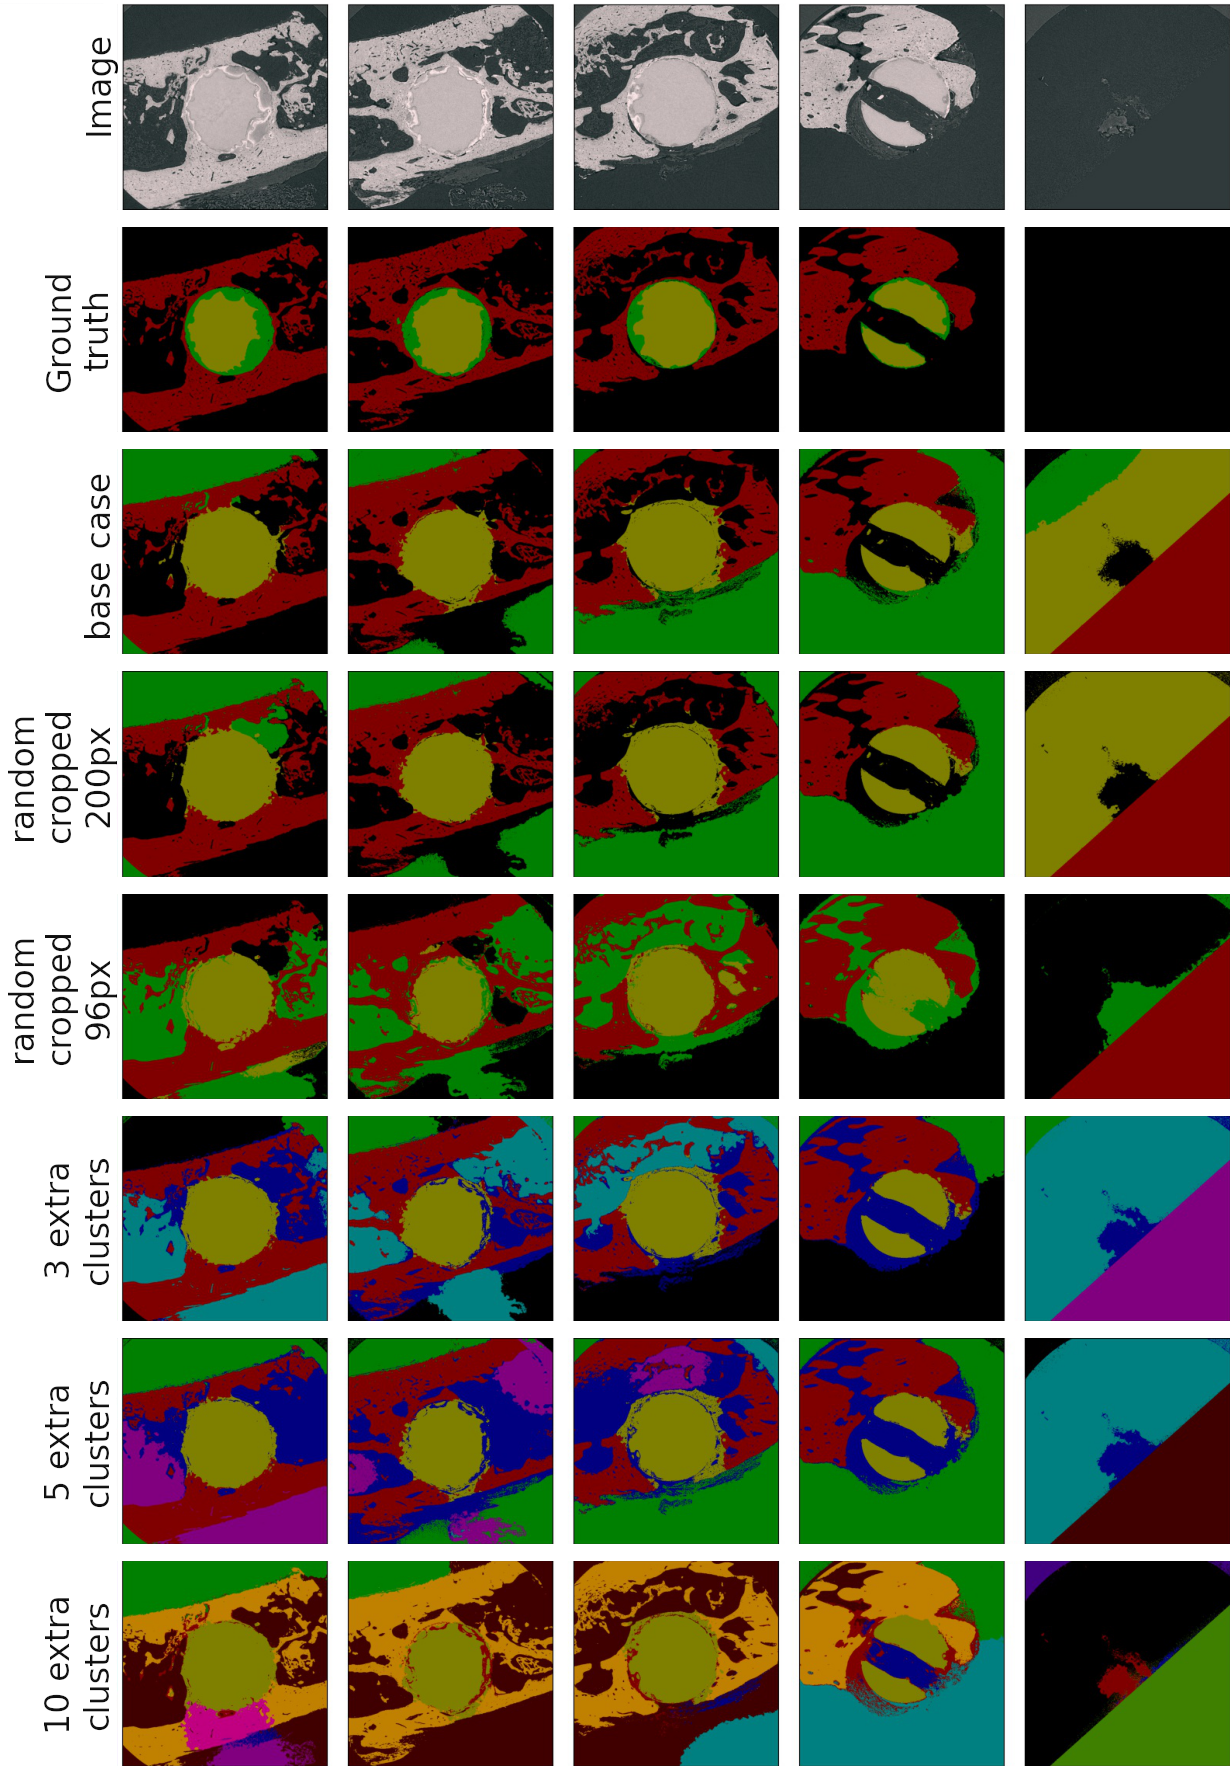
\includegraphics[width=\textwidth]{pictures/experiment_2/for_paper_all_experiments_example_predictions_2_Fold2}\\
    \caption[Comparison of Predictions for Same Fold]{Example predictions of Fold 2 of the base case, random cropping regimes, and overclustering regimes. For the overclustering regimes, the number of extra clusters is given. All shown slices belong to the second half of volume syn009HQ (which was neither part of train nor validation set) and are ordered according to spatial location in the volume. Every 100th slice is shown.}
    \label{fig:example-predictions-fold2}
\end{figure}
% contain the floats in this subsection
\FloatBarrier

\subsection{Discussion}
In this section, experiments will be discussed separately, followed by a comparison of results and a discussion of the potential of \gls{stego} for segmentation of scientific images.

\subsubsection{Experiment 1: Predict with Provided Models}
As expected, the pre-trained models did not perform well.
However, some resolution could be reached with all models, especially for \formatLabel{background}, where \gls{miou} was between 0.6 and 0.7.

%Potsdam
Potsdam only did a binary differentiation of \formatLabel{screw/degraded screw} from everything else.
However, even this separation is not distinguished very well, since often some nooks belonging to the bone and bone marrow are included (false positives).
The screw, in contrast, is always fully included in the label, no part is missing (few false negatives).
On the other hand, it does remarkably well on distinguishing the cracks in the screw, as seen in the example segmentations (\autoref{fig:pretrained-predictions}).
Overall, if the task was to only segment \formatLabel{screw/degraded screw} vs. \formatLabel{background}, this model would be not bad.
This means, that in the image features received from the backbone, there is something included, that can be used to identify screws.
%Potsdam was trained on aerial images, which are (in contrast to photographies on which the other models were trained), more similar to SRµCT pictures. So this might explain, why it performs better on the more laminary \formatLabel{screw} label.

% Cocostuff
With COCO-Stuff, most clusters mapped to the background of the sample, thus mostly \formatLabel{background} is predicted, with some segments of \formatLabel{bone} also identified correctly.
When \formatLabel{bone} was identified, it was usually correct, meaning that not many false positives were found.
However, \formatLabel{bone} was identified only where the depicted bone had a lighter color (a higher pixel value) and was very homogenous in the image, indicating that mostly pixel values were utilised for prediction.
%manual clustering
With the manual assignment of cluster 5 to \formatLabel{bone}, COCO-Stuff predictions did resemble the Cityscapes model more (in \gls{miou} as well as visually).
The biggest difference between these models then was, that COCO-Stuff yields more laminar clusters, with \formatLabel{bone} encompassing the full bone including matrix and screw, while the Cityscapes prediction is much more ragged and often neatly follows the lines of the bone marrow.


%Cityscapes
With Cityscapes, \formatLabel{background} and \formatLabel{bone} yielded similar \gls{miou} as predictions with COCO-Stuff.
However, as shown in the images, \formatLabel{bone} did correlate with the ground truth shape to a higher degree, which might indicate that only the border pixels differed.
As this might even be the case between two experts assigning the ground truth labels~\autocite{Webb2021}, the \gls{miou} might not be the best metric to choose for a comparison.
And as discussed in~\autocite{Reinke2022}, \gls{miou} especially is disadvantageous with close matches, since it does not differentiate between divergence at borders of regions or completely separate regions (for more details see~\autocite{Reinke2022}).
So overall, the Cityscapes model should be considered more effective than COCO-Stuff and also better than Potsdam at distinguishing \formatLabel{bone} from \formatLabel{background}, while Potsdam is more efficient at identifying \formatLabel{screw}.

% compare to paper results
In comparison to the model performance on the validation sets of the pre-trained models, it stands out that~–~with respect to \gls{miou}~–~the predictions on the screws data set are nearly as good as the validation results presented in the paper~\autocite{Hamilton2022}.
That means, prediction with an arbitrary selected model yielded similar results as predictions on the validation set of that model in terms of \gls{miou}.
However, when considering the actual predictions, it shows that they are very ineffective in comparison to the predictions of the validation set of the model.
Roughly the same proportions of pixels are in fact classified correctly as indicated by \gls{miou}, but especially borders between labels are often off, thus rendering the whole prediction pointless.
In comparison, the results on the original validation set do look more promising~\autocite{Hamilton2022}.
There, labels can be distinguished quite well and borders between labels often match at least in a broad sense~\autocite{Hamilton2022}.
This once again highlights the often deficient expressiveness of the \gls{miou}, as no differentiation is made between border pixels and others.
A more thorough discussion of the ~\gls{miou} (and other metrics) can be found in~\autocite{Reinke2022}.

% combination?
In combination, Potsdam and Cityscapes might yield acceptable results for the labels \formatLabel{background, bone}, and \formatLabel{screw} (e.g. by predicting after each other and merging \formatLabel{screw} pixels of Potsdam into \formatLabel{bone} pixels of Cityscapes).
However, a more promising approach would probably be to just train a new model for the screws data set.

% contain the floats in section
\afterpage{\FloatBarrier}

\subsubsection{Experiment 2: Train on Scientific Data Set}\label{subsubsec:discussion-experiment2}
In the following, the performance of the training regimes will be evaluated and compared to each other, as well as to the predictions made with the pre-trained models in experiment 1.
Especially the divergence between folds will be discussed, as well as the poor performance on the \formatLabel{degraded screw} label.
Eventually, recommendations for training \gls{stego} will be addressed.

%weight selection/tuning
As explained earlier, \gls{stego} requires six parameters of the loss function to be tuned depending on the training data used.
Tuning was done based on the recommendations by \gls{stego}s authors.
This means, the cosine distance signales were tuned to reach two distinct positive and negative signals, as illustrated in the segmentation correspondence histograms provided during training~\autocite{Hamilton2022}.
Originally, it was recommended to balance these signals to generate separated signals of approximately the same strength.
However, it turned out that slightly increasing the negative signal worked best for the used data, regardless of cropping regime and resolution\footnote{The full list of used parameters is found in \autoref{tab:training-parameters}.}.
A reason for this might be, that since the data set is very homogenous, with most slices showing the same view of the same objects over and over again, there is an imbalance in positive and negative signals.
Plenty of positive signal was provided from the similar images, but especially negative signal was rare.
That might be the reason why artificially shifting this balance towards negative signals was helpful.

% overall model performance
Overall, the models performed well, apart from the \formatLabel{degraded screw} label.
The differences between folds were minor.
Predictions on the validation set tend to be very similar: all models predict \formatLabel{bone} quite well, same goes for \formatLabel{screw} and \formatLabel{background}, while no model performs well on \formatLabel{degraded screw}.
The consistently poor performance of \formatLabel{degraded screw} highlights once again the challenging task to differentiate \formatLabel{degraded screw} from \formatLabel{screw}.
Since this label is so scarce, performance would considerably increase, when excluding \formatLabel{degraded screw} from the calculation of \gls{miou}.
This is impressively shown by the accuracy values, which are consistently higher than the \gls{miou} values, since they indicate the overall proportion of correctly classified pixels, while \gls{miou} is calculated as mean over labels, where all labels contribute equally.

% compare to predictions with pre-trained models
This relatively good performance of the models also shows in comparison with the predictions made with the pre-trained models, as the \gls{miou} nearly doubled.
Even though there were some labels, that did perform quite well in regard to \gls{iou} in the pre-trained models (for example \formatLabel{background}, where \gls{iou} was between 0.69 and 0.71), these predictions were far from good.
For example, the COCO-Stuff model, which yielded a \gls{iou} of 0.69 on \formatLabel{background}, nearly always predicted \formatLabel{background}.
So, the differentiating capacities were poor.\footnote{This again highlights the shortcomings of using the \gls{iou} as single metric for model evaluation (as discussed in~\autocite{Reinke2022}.}
Thus overall, it can be confirmed that training the segmentation head for specific tasks is beneficial and significantly improved model quality in comparison to arbitrary selected models.
However, the results for scientific data are still not satisfactory to be used in real-world scenarios.


% divergence of folds (and models)
As mentioned earlier, the development of the \gls{miou} diverges between folds in all trainings.
This might be attributed to the fact, that too few training examples were used, or that the models were not sufficiently tuned.
In the future, a more thorough parameter tuning should be done, possibly using grid search algorithms to find better parameters.
To investigate influence of data availability, training with the base case configuration was also done on five folds of a leave-one-out cross-validation.\footnote{Since it already showed, that divergence is present in a leave-one-out setting, too, training was stopped after five folds.}
%LOO
However, as seen in~\autoref{fig:miou-per-fold}, the divergence between folds was found in the leave-one-out cross-validation as well.
This indicates a higher variance between folds in the leave-one-out case, as it is often the case, when training sets are highly correlated~\autocite{Bengio2004}.
Overall, using a leave-one-out cross-validation did not improve model quality significantly.

%extra clusters
When overclustering was done, it was found that differentiation between bone and bone marrow, as well as between background and soft tissue, did improve visibly.
This is insofar remarkable, as this differentiation is not made in the ground truth, which highlights the potential of unsupervised algorithms, which are able to derive structures independently of the ground truth provided.

Concerning the \formatLabel{degraded screw} label, however, this label could not be retrieved, even when allowing for ten extra clusters.
Thus, it can be assumed, that at the current state of \gls{stego}, it seems not to be possible to retain this challenging label.
As \formatLabel{degraded screw} only slightly differs from \formatLabel{screw} in regard of absorption (and thus pixel values) or texture, it might be the case, that the feature vectors derived form the backbone did not differentiate these enough (meaning the feature embeddings are too similar to be clustered separately).
Thus, switching the backbone to something adapted for \gls{srmct} images should definitively be done in the future, to see if this helps feature embedding.
At least in principle, differentiating \formatLabel{screw} and \formatLabel{degraded screw} should be possible, as the \formatLabel{degraded screw} label has been successfully retained in another study~\autocite{Baltruschat2021}, which indicates, that there is something in the data, that can be used for differentiation (and it is very unlikely that it is just the label, that differentiates it).

%compare with supervised prediction
In comparison to this study~\autocite{Baltruschat2021}, which was done on the same data set, the results achieved here are worse.
However, it has to be noted, that the study was done with a supervised Network (a U-net), and also utilised 3D fusing, meaning predictions were done from multiple directions and combined by probability~\autocite{Baltruschat2021}.
Still, even without 3D fusing, results were significantly better: labels reached around 0.90~\gls{iou}, and even the \formatLabel{degraded screw} label reached 0.80~\autocite{Baltruschat2021}.

% very good for unsupervised
However, even though results are not ready to be used in a scientific real-world application, in the context of unsupervised segmentation, the achieved result is very good.
Most other unsupervised segmentation algorithms tend to reach a \gls{miou} of 0.12~to~0.31 (depending on the data set)~\autocite{Cho2021}, 0.21~\autocite{Hamilton2022}, or at best~0.50~to~0.63 (depending on number of classes)~\autocite{VanGansbeke2021} on default (2D) image data sets.

% RESULT: How to train SRµCT data?
The remaining problem to be solved is, that no clear recommendation regarding the cropping scheme could be derived from the experiments presented, due to the divergence during cross validation.
Overall, the base case was found to perform slightly better than the random cropped regimes in regard to \gls{miou}, which was 0.47 (mean over folds), single folds even reached scores of 0.49 or 0.50.
The base case was also found to yield the best \gls{miou} scores (mean over folds) for \formatLabel{background} and \formatLabel{bone} (0.59 and 0.69 respectively) and the second best for \formatLabel{screw} (0.61)\footnote{Leave-one-out cross-validation is excluded from this comparison, since not all folds were trained.}.
It also did diverge less between folds.
But again, these differences were only minor compared to the other cropping regimes, and similar differences between models were even found between folds of the base case.
However, all models were able to predict the labels to some degree.
Finally, this means, that the idea of a heterogeneous data set (as generated through random cropping) being more beneficial when training \gls{stego}, could not be confirmed.
Since results of all trainings are very similar regarding the final model and training times until the best model is found, did not differ a lot (1.5~to 5~hours), there is no definite answer to which cropping regime and resolution to prefer.
As the \gls{miou} curves of the random cropped regimes do not fluctuate as much (and especially performance does not decrease as much over time), it might be preferred over the base case.
Especially, since it can be suspected that these trainings might even improve with further training (for example fold~1 on 96~px random cropped,~\autoref{fig:miou-per-fold-label}), random cropping might be advantageous, as training these for longer still results in reasonable training times (20 epochs took only 4.5~h and 1.5~h).


\subsubsection{Potential of STEGO for Scientific Segmentation}
% compare to stegos performance on default sets and wrap up
In a broader view, it is remarkable how well \gls{stego} performed on the \gls{srmct} data, for which it was never designed.
When comparing the results with those of the original trainings done on photography based data sets, the \gls{miou} nearly doubled.
This might largely be attributed to the fact, that through training on very similar images, which always depict the same object, the number of training examples per label is very high.
But given that \gls{stego} was used for scientific segmentation, which it was not designed for, and with a backbone that was also not designed for scientific images, the results are very good.
Achieving these promising results with such an unsuitable backbone highlights the potential \gls{stego} has to be adapted for unsupervised semantic segmentation of scientific images.


\subsubsection{Future Work}
This paper does only provide a very broad evaluation of \gls{stego}.
Especially to give better recommendations for training \gls{stego} on scientific images, more research is needed.

% train backbone
The factor that probably has the most influence is the backbone, which was frozen and not trained in any capacity.
This backbone was originally trained on photographs~\autocite{Hamilton2022,Caron2021} and was not adjusted for ~\gls{srmct} images.
As stated in~\autocite{Cheplygina2019}, even though ImageNet is often used in transfer learning set-ups for medical images, this is largely attributed to its availability, as there are only few alternative so readily available.
Even though correlation correspondence was promising (as shown in~\autoref{fig:correspondencemap-screws}), training the backbone specifically on \gls{srmct} data might significantly enhance feature embedding of the output, which in turn should be easier to cluster by the segmentation head.
So in the long run, it should be investigated, if training the backbone enhances results.

% parameter tuning
Additionally, a systematic grid search to optimise training parameters might also improve the results.
There could even be parameter combinations, that mitigate the divergence between folds or significantly improve resolution of the \formatLabel{degraded screw} label.
% more data
%In that regard, trainings done on more data can also be helpful.

% other grey value normalisation
Also the used pixel-value normalisation scheme should be investigated further, since the used scheme still relies on mean and standard deviation derived from photographs.
Adapting the normalisation scheme to the respective imaging modality could also enhance the feature quality derived from the backbone.

%% other modalities
Generally, working with more and different data should also be evaluated, since a single \gls{srmct} data set is not representative for scientific imaging at all.
Even combining different data sets of both the same and different imaging modalities to enhance data and label heterogeneity might help.
%stegos potential is not fully utilised in this study
And it was not even tried in this study to utilise the 3D information embedded in the data set.
Future research might aim at integrating the 3D aspect, for example by using slices from different directions for training and combining final 3D predictions from single slice predictions of different directions, as done in~\autocite{Zhou2017}.

